%
% BA Sachsen - StA Dresden
%
% LaTeX-Vorlage für Abschlussarbeiten im Bereich Technik
%
%
% Erstellt von Tenshi Hara und bereitgestellt unter einer
%
%       GNU Public License, Version 3 (GPLv3)
%
% Näheres zur Lizenz entnehmen Sie der Datei Lizenz.txt.
% Sollten Sie diese Vorlage ohne die Lizenz-Datei erhalten
% haben, informieren Sie bitte die Free Software Foundation.
%
%%%%%%%%%%%%%%%%%%%%%%%%%%%%%%%%%%%%%%%%%%%%%%%%%%%%%%%%%%%%%%
%

%
% Die folgenden beiden Zeilen können Sie auskommentieren,
% da sie nur eine störende Warning unterdrücken.
%
\RequirePackage{silence}
\WarningFilter{remreset}{The remreset package}

%
% Eigentlicher Beginn des Dokuments
%
\documentclass[a4paper,
pagebackref, % auskommentieren, falls Sie BibLaTeX benutzen
twoside, % auskommentieren, falls Sie einseitig binden wollen
% Die folgende Zeile einkommentieren, falls Sie ein PDF-A benötigen
% pdfa,pdfapart=2,pdfaconformance=A,extension=pdf
]{book}
\usepackage[utf8]{inputenc}
\usepackage{lmodern}
\usepackage[T1]{fontenc}
\usepackage{ifthen}

%
% Alle Anpassungen der Titelseite erledigen Sie in der folgenden Datei
%
%
% BA Sachsen - StA Dresden
%
% LaTeX-Vorlage für Abschlussarbeiten im Bereich Technik
%
%
% Erstellt von Tenshi Hara und bereitgestellt unter einer
%
%       GNU Public License, Version 3 (GPLv3)
%
% Näheres zur Lizenz entnehmen Sie der Datei Lizenz.txt.
% Sollten Sie diese Vorlage ohne die Lizenz-Datei erhalten
% haben, informieren Sie bitte die Free Software Foundation.
%
%%%%%%%%%%%%%%%%%%%%%%%%%%%%%%%%%%%%%%%%%%%%%%%%%%%%%%%%%%%%%%
%
% Vorlage nutzt BibTeX. Falls Sie BibLaTeX benutzen wollen,
% scrollen Sie ans Ende dieser Datei und beachten Sie die
% Hinweise dort.
%
%%%%%%%%%%%%%%%%%%%%%%%%%%%%%%%%%%%%%%%%%%%%%%%%%%%%%%%%%%%%%%
%
% Zufrieden? ---> https://ko-fi.com/tchara
%
%%%%%%%%%%%%%%%%%%%%%%%%%%%%%%%%%%%%%%%%%%%%%%%%%%%%%%%%%%%%%%
%
% 1. Personendaten
%
\newcommand{\myTitle}{Empfehlung für die Gestaltung wissenschaftlicher Ausarbeitungen im Studienbereich Technik, insbesondere den Ingenieurwissenschaften}
\newcommand{\mySubtitle}{Vorlage für die Bachelor-Arbeit}
\newcommand{\myDegree}{Bachelor of Engineering}
\newcommand{\myDegreeShort}{B.Eng.}
\newcommand{\myName}{Paris Studiumsmensch}
\newcommand{\myCompany}{Praxisgesellschaft mbH \& Co KG}
\newcommand{\myCompanyAddress}{Musterstraße 1, 01001 Dresden}
\newcommand{\myId}{3012345}
\newcommand{\myExpert}{Dipl.-Ing. Kader Praxismensch}
\newcommand{\myProf}{Prof. Dr.-Ing. Arin Schlaumeier}
\newcommand{\myAcademy}{Staatliche Studienakademie Dresden}
% Vorsicht mit den Begriffen „Studiengang“ und „Studienrichtung“!
\newcommand{\myStudy}{Studienrichtung Informationstechnik}
\newcommand{\myLocation}{Dresden} 
\newcommand{\myVersion}{Version 1.0}
% Abgabedatum
\newcommand{\mySubmissionDate}{22. Juli 202X}
% Datum der Selbständigkeitserklärung
% Abgabedatum und Datum der Selbständigkeitserklärung müssen nicht
% zwingend identisch sein. Sie können die Erklärung bereits ein paar
% Tage vorher (beispielsweise direkt nach dem Drucken und Binden)
% unterschreiben, während Sie die Arbeit erst später einreichen.
\newcommand{\myDeclarationDate}{20. Juli 202X}

%
% 2. Konfiguration
%
% 2a) Hat diese Arbeit einen Sperrvermerk?
%
\newboolean{lockflag}
\setboolean{lockflag}{true} % „false“, falls kein Sperrvermerk
%
% 2b) Soll statt des Abstracts ein Autorenreferat erscheinen?
%
\newboolean{extendedabstract}
\setboolean{extendedabstract}{false} % „true“, falls Autorenreferat

%
% 3. gescanntes Auftragsblatt einfügen
%
\newboolean{auftragsblatt}
\setboolean{auftragsblatt}{true}
% "false", falls kein Auftragsblatt eingebaut werden soll.
% Das Auftragsblatt muss sowohl im Printexemplar als auch in der
% elektronischen Version eingebunden werden! - In dieser Vorlage
% ist dafür der Platz zwischen der Zusammenfassung und dem
% Inhaltsverzeichnis vorgesehen.
% Für die elektronische Version bietet sich das Einbinden eines
% Scans an (true).
% Für die Printexemplare sollten Sie die Seitenzähler einfach nur
% um 2 erhöhen (true) und dann später die entsprechenden Blätter
% einlegen:
% * das Pflichtexemplar für das Archiv erhält das Original
% * die anderen Exemplare eine Kopie

%
% 4. Lorem Ipsum (am Ende auskommentieren!)
%
\usepackage{lipsum}

%
% 5. zu verwendende Pakete
%
% Hinweise zur Geometrie im Dokument beachten!
\usepackage{geometry}
\geometry{
    inner=40mm,
    outer=30mm,
    top=30mm
}
% Setzen Sie im folgenden die Option „htt“, wenn Sie wollen, dass
% Text in den Umgebungen \texttt und \ttfamily auch den Trennregeln
% des hyphenat-Pakets unterliegen sollen.
%\usepackage[htt]{hyphenat}
\usepackage{hyphenat}
\usepackage[ngerman,english]{babel}
\usepackage[babel]{csquotes}
\usepackage{cite}
\usepackage{amsmath,amssymb,amstext,amsthm}
\usepackage{upgreek,units}
\usepackage{listings}
\lstset{ %
	basicstyle=\small,		% Schriftgröße im Kodeblock
	numberstyle=\tiny,
	numbers=left,			% Position der Zeilennummern
	stepnumber=1,			% Schrittweite der Zeilennummern („1“ bedeutet jede Zeile wird beschriftet)
	frame=tbl,				% Rahmen um Kodeblock (Standard: „single“)
	xleftmargin=15pt,
	numbersep=10pt,
	tabsize=4,				% Tabulatorgröße (4 Leerzeichen)
	captionpos=t,			% Position der Beschriftung
	breaklines=true,		% automatischer Zeilenumbruch
	breakatwhitespace=true,	% automatischer Zeilenumbruch nur an Leerzeichen, Tabulatoren, etc.
}
\renewcommand{\lstlistingname}{Quellkode}
\lstdefinestyle{plain}{frame=single, breaklines=true}
\lstdefinestyle{Java}{language=Java, basicstyle=\small, numbers=left, numberstyle=\tiny, numberblanklines=false, tabsize=4, xleftmargin=1.6em, frame=single, breaklines=true}
\usepackage{graphicx}
\usepackage{caption,subcaption}

\usepackage[hang,multiple]{footmisc}
\renewcommand{\footnotemargin}{1.2em}
\usepackage{longtable,booktabs,multirow,colortbl}
\usepackage{rotating}
\usepackage{remreset}
\usepackage{savefnmark}
\usepackage{enumerate}
\usepackage[shortlabels]{enumitem}
\setlist{noitemsep, itemsep=3pt, topsep=0pt, partopsep=6pt}
\setenumerate{noitemsep, itemsep=3pt, topsep=0pt, partopsep=6pt}

\usepackage{thmtools}
\usepackage[nothm]{thmbox}
\usepackage[mathscr]{eucal}
\newtheoremstyle{style}
	{0}									%	Platz drüber
	{0}									%	Platz drunter
	{\normalfont}						%	Schriftstil
	{}									%	Einrückung
	{\normalfont\bfseries}				%	Theorembezeichner-Stil
	{:\\\vphantom{-}\vspace*{-.75em}\\}	%	Trennzeichen Bezeichner --> Inhalt
	{5pt plus 1pt minus 1pt}			%	Trennzeichen Text --> Theorem
	{{\normalfont\bfseries \thmname{#1}\thmnumber{ #2}\thmnote{ (#3)}}}
\theoremstyle{style}

\definecolor{HKS41-100}{cmyk}{1.0, 0.7, 0.1, 0.5}
\definecolor{HKS41-90}{cmyk}{0.9, 0.63, 0.09, 0.45}
\definecolor{HKS41-80}{cmyk}{0.8, 0.56, 0.08, 0.4}
\definecolor{HKS41-70}{cmyk}{0.7, 0.49, 0.07, 0.35}
\definecolor{HKS41-60}{cmyk}{0.6, 0.42, 0.06, 0.3}
\definecolor{HKS41-50}{cmyk}{0.5, 0.35, 0.05, 0.25}
\definecolor{HKS41-40}{cmyk}{0.4, 0.28, 0.04, 0.2}
\definecolor{HKS41-30}{cmyk}{0.3, 0.21, 0.03, 0.15}
\definecolor{HKS41-20}{cmyk}{0.2, 0.14, 0.02, 0.1}
\definecolor{HKS41-10}{cmyk}{0.1, 0.07, 0.01, 0.05}
\definecolor{HKS44-100}{cmyk}{1.0, 0.5, 0.0, 0.0}
\definecolor{HKS44-90}{cmyk}{0.9, 0.45, 0.0, 0.0}
\definecolor{HKS44-80}{cmyk}{0.8, 0.4, 0.0, 0.0}
\definecolor{HKS44-70}{cmyk}{0.7, 0.35, 0.0, 0.0}
\definecolor{HKS44-60}{cmyk}{0.6, 0.3, 0.0, 0.0}
\definecolor{HKS44-50}{cmyk}{0.5, 0.25, 0.0, 0.0}
\definecolor{HKS44-40}{cmyk}{0.4, 0.2, 0.0, 0.0}
\definecolor{HKS44-30}{cmyk}{0.3, 0.15, 0.0, 0.0}
\definecolor{HKS44-20}{cmyk}{0.2, 0.1, 0.0, 0.0}
\definecolor{HKS44-10}{cmyk}{0.1, 0.05, 0.0, 0.0}
\definecolor{HKS36-100}{cmyk}{0.8, 0.9, 0.0, 0.0}
\definecolor{HKS36-90}{cmyk}{0.72, 0.81, 0.0, 0.0}
\definecolor{HKS36-80}{cmyk}{0.64, 0.72, 0.0, 0.0}
\definecolor{HKS36-70}{cmyk}{0.56, 0.63, 0.0, 0.0}
\definecolor{HKS36-60}{cmyk}{0.48, 0.54, 0.0, 0.0}
\definecolor{HKS36-50}{cmyk}{0.4, 0.45, 0.0, 0.0}
\definecolor{HKS36-40}{cmyk}{0.32, 0.36, 0.0, 0.0}
\definecolor{HKS36-30}{cmyk}{0.24, 0.27, 0.0, 0.0}
\definecolor{HKS36-20}{cmyk}{0.16, 0.18, 0.0, 0.0}
\definecolor{HKS36-10}{cmyk}{0.08, 0.09, 0.0, 0.0}
\definecolor{HKS33-100}{cmyk}{0.5, 1.0, 0.0, 0.0}
\definecolor{HKS33-90}{cmyk}{0.45, 0.9, 0.0, 0.0}
\definecolor{HKS33-80}{cmyk}{0.4, 0.8, 0.0, 0.0}
\definecolor{HKS33-70}{cmyk}{0.35, 0.7, 0.0, 0.0}
\definecolor{HKS33-60}{cmyk}{0.3, 0.6, 0.0, 0.0}
\definecolor{HKS33-50}{cmyk}{0.25, 0.5, 0.0, 0.0}
\definecolor{HKS33-40}{cmyk}{0.2, 0.4, 0.0, 0.0}
\definecolor{HKS33-30}{cmyk}{0.15, 0.3, 0.0, 0.0}
\definecolor{HKS33-20}{cmyk}{0.1, 0.2, 0.0, 0.0}
\definecolor{HKS33-10}{cmyk}{0.05, 0.1, 0.0, 0.0}
\definecolor{HKS57-100}{cmyk}{1.0, 0.0, 0.9, 0.2}
\definecolor{HKS57-90}{cmyk}{0.9, 0.0, 0.81, 0.18}
\definecolor{HKS57-80}{cmyk}{0.8, 0.0, 0.72, 0.16}
\definecolor{HKS57-70}{cmyk}{0.7, 0.0, 0.63, 0.14}
\definecolor{HKS57-60}{cmyk}{0.6, 0.0, 0.54, 0.12}
\definecolor{HKS57-50}{cmyk}{0.5, 0.0, 0.45, 0.1}
\definecolor{HKS57-40}{cmyk}{0.4, 0.0, 0.36, 0.08}
\definecolor{HKS57-30}{cmyk}{0.3, 0.0, 0.27, 0.06}
\definecolor{HKS57-20}{cmyk}{0.2, 0.0, 0.18, 0.04}
\definecolor{HKS57-10}{cmyk}{0.1, 0.0, 0.09, 0.02}
\definecolor{HKS65-100}{cmyk}{0.65, 0.0, 1.0, 0.0}
\definecolor{HKS65-90}{cmyk}{0.585, 0.0, 0.9, 0.0}
\definecolor{HKS65-80}{cmyk}{0.52, 0.0, 0.8, 0.0}
\definecolor{HKS65-70}{cmyk}{0.455, 0.0, 0.7, 0.0}
\definecolor{HKS65-60}{cmyk}{0.39, 0.0, 0.6, 0.0}
\definecolor{HKS65-50}{cmyk}{0.325, 0.0, 0.5, 0.0}
\definecolor{HKS65-40}{cmyk}{0.26, 0.0, 0.4, 0.0}
\definecolor{HKS65-30}{cmyk}{0.195, 0.0, 0.3, 0.0}
\definecolor{HKS65-20}{cmyk}{0.13, 0.0, 0.2, 0.0}
\definecolor{HKS65-10}{cmyk}{0.065, 0.0, 0.1, 0.0}
\definecolor{HKS07-100}{cmyk}{0.0, 0.6, 1.0, 0.0}
\definecolor{HKS07-90}{cmyk}{0.0, 0.54, 0.9, 0.0}
\definecolor{HKS07-80}{cmyk}{0.0, 0.48, 0.8, 0.0}
\definecolor{HKS07-70}{cmyk}{0.0, 0.42, 0.7, 0.0}
\definecolor{HKS07-60}{cmyk}{0.0, 0.36, 0.6, 0.0}
\definecolor{HKS07-50}{cmyk}{0.0, 0.3, 0.5, 0.0}
\definecolor{HKS07-40}{cmyk}{0.0, 0.24, 0.4, 0.0}
\definecolor{HKS07-30}{cmyk}{0.0, 0.18, 0.3, 0.0}
\definecolor{HKS07-20}{cmyk}{0.0, 0.12, 0.2, 0.0}
\definecolor{HKS07-10}{cmyk}{0.0, 0.06, 0.1, 0.0}
\definecolor{HKS14-100}{cmyk}{0.0, 1.0, 1.0, 0.0}
% Benannte Farben
\definecolor{white}{gray}{1.00}
\definecolor{black}{gray}{0.00}
\definecolor{skyblue}{cmyk}{0.4, 0.2, 0.0, 0.0}             % HKS44-40
\definecolor{blue}{cmyk}{1.0, 0.5, 0.0, 0.0}                % HKS44-100
\definecolor{lightblue}{cmyk}{0.7, 0.35, 0.0, 0.0}          % HKS44-70
\definecolor{darkblue}{rgb}{0.04, 0.16, 0.32}               % 
\definecolor{extradarkblue}{cmyk}{1.00, 0.70, 0.10, 0.50}   % HKS41-100
\definecolor{darkgreen}{cmyk}{1.0, 0.0, 0.9, 0.2}           % HKS57-100
\definecolor{green}{cmyk}{0.65, 0.0, 1.0, 0.0}              % HKS65-100
\definecolor{purple}{cmyk}{0.5, 1.0, 0.0, 0.0}              % HKS33-100
\definecolor{indigo}{cmyk}{0.8, 0.9, 0.0, 0.0}              % HKS36-100
\definecolor{gray}{gray}{0.59}
\definecolor{darkgray}{gray}{0.50}
\definecolor{darkcyan}{cmyk}{0.87, 0.4, 0.4, 0.0}
\definecolor{cyan}{cmyk}{0.78, 0.19, 0.01, 0.0}
\definecolor{lightcyan}{cmyk}{0.39, 0.095, 0.005, 0.0}
\definecolor{extralightcyan}{cmyk}{0.16, 0.1, 0.0, 0.0}
    
\definecolor{shadeThe}{cmyk}{.1,.05,0,0}		% HKS44_10%
\definecolor{frameThe}{cmyk}{.7,.35,0,0}		% HKS44_70%
\definecolor{shadeDef}{cmyk}{.07,0,.1,0}		% HKS65_10%
\definecolor{frameDef}{cmyk}{.2,0,.4,0}			% HKS65_40%
\definecolor{shadeThm}{cmyk}{.05,.1,0,0}		% HKS33_10%
\definecolor{frameThm}{cmyk}{.2,.4,0,0}			% HKS33_40%
\definecolor{shadeLem}{cmyk}{0,.06,.1,0}		% HKS07_10%
\definecolor{frameLem}{cmyk}{0,.24,.4,0}		% HKS07_40%
\definecolor{shadeCor}{cmyk}{.1,.07,.01,.05}	% HKS41_10%
\definecolor{frameCor}{cmyk}{.4,.28,.04,.2}		% HKS41_40%
\definecolor{shadePrf}{cmyk}{.08,.09,0,0}		% HKS36_10%
\definecolor{framePrf}{cmyk}{.32,.36,0,0}		% HKS36_40%
\definecolor{shadeAss}{cmyk}{.1,0,.09,.02}		% HKS57_10%
\definecolor{frameAss}{cmyk}{.34,0,.36,.08}		% HKS57_40%

\declaretheorem[name=Arbeitsthese,shaded={rulecolor=frameThe,rulewidth=1pt,bgcolor=shadeThe,textwidth=\textwidth-2pt}]{myworkingthesis}
\declaretheorem[name=Annahme,numbered=no,shaded={rulecolor=frameAss,rulewidth=1pt,bgcolor=shadeAss,textwidth=\textwidth-2pt}]{myassertion}
\declaretheorem[numberwithin=section,name=Definition,shaded={rulecolor=frameDef,rulewidth=1pt,bgcolor=shadeDef,textwidth=\textwidth-2pt}]{mydef}
\declaretheorem[sibling=mydef,name=Theorem,shaded={rulecolor=frameThm,rulewidth=1pt,bgcolor=shadeThm,textwidth=\textwidth-2pt}]{mytheorem}
\declaretheorem[sibling=mydef,name=Lemma,shaded={rulecolor=frameLem,rulewidth=1pt,bgcolor=shadeLem,textwidth=\textwidth-2pt}]{mylemma}
\declaretheorem[sibling=mydef,name=Korollar,shaded={rulecolor=frameCor,rulewidth=1pt,bgcolor=shadeCor,textwidth=\textwidth-2pt}]{mycorollary}
\declaretheorem[sibling=mydef,name=Beweis,shaded={rulecolor=framePrf,rulewidth=1pt,bgcolor=shadePrf,textwidth=\textwidth-2pt}]{myproof}
\declaretheorem[sibling=mydef,name=Abbildung]{myfig}

\AtBeginDocument{\numberwithin{lstlisting}{section}}
\newcounter{thmhelper}[section]
\newcounter{thesiscount}
\makeatletter
	\@removefromreset{footnote}{chapter}
\makeatother

\usepackage{wrapfig}

\newcommand{\inlinecode}[1]{%
    \colorbox{extralightcyan}{%
        \texttt{#1}%
    }%
}%

\newcommand{\mytable}[0]{%
	\setcounter{table}{\thethmhelper}%
	\addtocounter{thmhelper}{1}%
	}{%
}%
\newcommand{\myequation}[0]{%
	\setcounter{equation}{\thethmhelper}%
	\addtocounter{thmhelper}{1}%
	}{%
}%
\newenvironment{workingthesis}[1][]{%
	\addtocounter{thesiscount}{1}%
	\begin{myworkingthesis}[#1]}{\end{myworkingthesis}%
}%
\newenvironment{assertion}[1][]{%
	\begin{myassertion}[#1]}{\end{myassertion}%
}%
\newenvironment{definition}[1][]{%
	\addtocounter{thmhelper}{1}%
	\begin{mydef}[#1]}{\end{mydef}%
}%
\newenvironment{theorem}[1][]{%
	\addtocounter{thmhelper}{1}%
	\begin{mytheorem}[#1]}{\end{mytheorem}%
}%
\newenvironment{lemma}[1][]{%
	\addtocounter{thmhelper}{1}%
	\begin{mylemma}[#1]}{\end{mylemma}%
}%
\newenvironment{corollary}[1][]{%
	\addtocounter{thmhelper}{1}%
	\begin{mycorollary}[#1]}{\end{mycorollary}%
}%
\renewenvironment{proof}[1][]{%
	\addtocounter{thmhelper}{1}%
	\begin{myproof}[#1]}{%
		\nopagebreak%
		\\%
		{} \qed%
	\end{myproof}%
}%
\newcommand{\comment}[1]{%
	\, {} \hfill {\, }%
	{\color{gray}\begin{thmbox}[S]{\textit{Kommentar}}%
		\setlength{\parindent}{-0.3em}%
		\textit{#1}%
	\end{thmbox}}%
	\vspace{1em}%
}%
\renewcommand{\example}[1]{%
	\, {} \hfill {\, }%
	\begin{thmbox}[S]{\textit{Beispiel}}%
		\setlength{\parindent}{-0.2em}%
		#1%
	\end{thmbox}%
	\vspace{1em}%
}%

% Paket catoptions ist defekt; für Optionen in ASCII-Zeichen
% muss händisch korrigiert werden
% \usepackage{catoptions}

\makeatletter%
	\def\Autoref#1{%
		\begingroup%
			\def\reserved@a{\cpttrimspaces{#1}}%
			\ifcsndefTF{r@#1}{%
				\xaftercsname{\expandafter\testreftype\@fourthoffive}%
				{r@\reserved@a}.\\{#1}%
			}{%
				\ref{#1}%
			}%
		\endgroup%
	}%
	\def\testreftype#1.#2\\#3{%
		\ifcsndefTF{#1autorefname}{%
			\def\reserved@a##1##2\@nil{%
				\uppercase{\def\ref@name{##1}}%
				\csn@edef{#1autorefname}{\ref@name##2}%
				\autoref{#3}%
			}%
			\reserved@a#1\@nil%
		}{%
			\autoref{#3}%
		}%
	}%
\makeatother%

\usepackage{imakeidx}
\makeindex

\usepackage{xr-hyper}
\usepackage{hyperxmp}
\numberwithin{figure}{section}
\numberwithin{table}{section}
\numberwithin{table}{section}
\numberwithin{equation}{section}
\addto\extrasngerman{%
    \renewcommand{\figureautorefname}{Abbildung}
    \renewcommand{\tableautorefname}{Tabelle}
	\renewcommand{\subsectionautorefname}{Unterabschnitt}%
	\renewcommand{\sectionautorefname}{Abschnitt}%
	\renewcommand{\chapterautorefname}{Kapitel}%
	\renewcommand{\partautorefname}{Teil}%
}
\pagecolor{white}
\usepackage{pdfpages}
\newcommand{\imgbox}[7]{%
	\begin{wrapfigure}{#1}{#2}%
		\centering%
		\vspace{-0.5em}%
		\includegraphics[width=#3]{figures/#4}%
		\vspace{-1.0em}%
		\setcounter{figure}{\thethmhelper}%
		\addtocounter{thmhelper}{1}%
		\caption[#6]{#7}\label{fig:#5}%
		\vspace{-0.5em}%
	\end{wrapfigure}%
}%
\newcommand{\img}[5]{%
	\begin{figure}[htbp]%
	%% zwei Abbildungen nebeneinander
    %%  #1 Breite der Abbildung
	%%  #2 Abbildung
	%%  #3 Label
	%%  #4 TOC-Beschriftung
	%%  #5 Beschriftung
	%%
	%% (Falls es komisch aussieht, setzen Sie
	%%  nur „t“ oder „tb“ statt „htbp“)
		\vspace{2.5em}%
		\centering%
		\includegraphics[width=#1]{figures/#2}
		\vspace{-0.5em}%
		\setcounter{figure}{\thethmhelper}%
		\addtocounter{thmhelper}{1}%
		\caption[#4]{#5}\label{fig:#3}%
		\vspace{1.5em}%
		\end{figure}%
}%
\newcommand\imgAB[9]{%
	%% LaTeX-Hexerei mit \imgABcontinued
	%% (wegen mehr als 9 Parametern)
	\def\tmpvalone{#1}%
	\def\tmpvaltwo{#2}%
	\def\tmpvalthr{#3}%
	\def\tmpvalfou{#4}%
	\def\tmpvalfiv{#5}%
	\def\tmpvalsix{#6}%
	\def\tmpvalsev{#7}%
	\def\tmpvaleig{#8}%
	\def\tmpvalnin{#9}%
	\imgABcontinued%
}%
\newcommand{\imgABcontinued}[2]{%
	\begin{figure}[htbp]%
	%% zwei Abbildungen nebeneinander
    %%  #1 Label des Containers
	%%  #2 TOC-Beschriftung des Containers
	%%  #3 Beschriftung des Containers
	%%  #4 Breite des linken Containers (A)
	%%  #5 Breite der Abbildung in A
	%%  #6 Abbildung in A
	%%  #7 Beschriftung in A
	%%  #8 Breite des rechten Containers (B)
	%%  #9 Breite der Abbildung in B
	%% #10 Abbildung in B
	%% #11 Beschriftung in B
	%%
	%% (Falls es komisch aussieht, setzen Sie
	%%  nur „t“ oder „tb“ statt „htbp“)
		\vspace{2.5em}%
		\centering%
		\begin{subfigure}[t]{\tmpvalfou\textwidth}%
			\centering%
			\includegraphics[width=\tmpvalfiv]{figures/\tmpvalsix}%
			\caption{\tmpvalsev}\label{fig:\tmpvalone-A}%
		\end{subfigure}%
		\hfill~%
		\begin{subfigure}[t]{\tmpvaleig\textwidth}%
			\centering%
			\includegraphics[width=\tmpvalnin]{figures/#1}%
			\caption{#2}\label{fig:\tmpvalone-B}%
		\end{subfigure}%
		\vspace{-0.5em}%
		\addtocounter{thmhelper}{1}%
		\setcounter{figure}{\thethmhelper}%
		\caption[\tmpvaltwo]{\tmpvalthr}\label{fig:\tmpvalone}%
		\vspace{1.5em}%
	\end{figure}%
}%
\newcommand{\imgABstack}[9]{%
	\begin{figure}[htbp]%
	%% zwei Abbildungen untereinander
	%% #1 Label des Containers
	%% #2 TOC-Beschriftung des Containers
	%% #3 Beschriftung des Containers
	%% #4 Breite der oberen Abbildung (A)
	%% #5 obere Abbildung (A)
	%% #6 Beschriftung der oberen Abbildung (A)
	%% #7 Breite der unteren Abbildung (B)
	%% #8 untere Abbildung (B)
	%% #9 Beschriftung der unteren Abbildung (B)
	%%
	%% (Falls es komisch aussieht, setzen Sie
	%%  nur „t“ oder „tb“ statt „htbp“)
		\vspace{2.5em}%
		\centering%
		\begin{subfigure}[t]{\textwidth}%
			\centering%
			\includegraphics[width=#4]{figures/#5}%
			\caption{#6}\label{fig:#1-A}%
		\end{subfigure}%
		\\%
		\vspace{2em}%
		\begin{subfigure}[t]{\textwidth}%
			\centering%
			\includegraphics[width=#7]{figures/#8}%
			\caption{#9}\label{fig:#1-B}%
		\end{subfigure}%
		\vspace{-0.5em}%
		\addtocounter{thmhelper}{1}%
		\setcounter{figure}{\thethmhelper}%
		\caption[#2]{#3}\label{fig:#1}%
		\vspace{1.5em}%
	\end{figure}%
}%
\newcommand\imgABC[9]{%
	%% LaTeX-Hexerei mit \imgABCcontinued
	%% (wegen mehr als 9 Parametern)
	\def\tmpvalone{#1}%
	\def\tmpvaltwo{#2}%
	\def\tmpvalthr{#3}%
	\def\tmpvalfou{#4}%
	\def\tmpvalfiv{#5}%
	\def\tmpvalsix{#6}%
	\def\tmpvalsev{#7}%
	\def\tmpvaleig{#8}%
	\def\tmpvalnin{#9}%
	\imgABCcontinued%
}%
\newcommand{\imgABCcontinued}[3]{%
	\begin{figure}[htbp]%
	%% drei Abbildungen nebeneinander
    %% #1 Label des Containers
	%% #2 TOC-Beschriftung des Containers
	%% #3 Beschriftung des Containers
	%% #4 Breite der linken Abbildung (A)
	%% #5 linke Abbildung (A)
	%% #6 Beschriftung der linken Abbildung (A)
	%% #7 Breite der mittleren Abbildung (B)
	%% #8 mittlere Abbildung (B)
	%% #9 Beschriftung der mittleren Abbildung (B)
	%% #10 Breite der rechten Abbildung (C)
	%% #11 rechte Abbildung (C)
	%% #12 Beschriftung der rechten Abbildung (C)
	%%
	%% (Falls es komisch aussieht, setzen Sie
	%%  nur „t“ oder „tb“ statt „htbp“)
		\vspace{2.5em}%
		\centering%
		\begin{subfigure}[t]{0.3\textwidth}%
			\centering%
			\includegraphics[width=\tmpvalfou]{figures/\tmpvalfiv}%
			\caption{\tmpvalsix}\label{fig:\tmpvalone-A}%
		\end{subfigure}%
		\hfill~%
		\begin{subfigure}[t]{0.3\textwidth}%
			\centering%
			\includegraphics[width=\tmpvalsev]{figures/\tmpvaleig}%
			\caption{\tmpvalnin}\label{fig:\tmpvalone-B}%
		\end{subfigure}%
		\hfill~%
		\begin{subfigure}[t]{0.3\textwidth}%
			\centering%
			\includegraphics[width=#1]{figures/#2}%
			\caption{#3}\label{fig:\tmpvalone-C}%
		\end{subfigure}%
		\vspace{-0.5em}%
		\addtocounter{thmhelper}{1}%
		\setcounter{figure}{\thethmhelper}%
		\caption[\tmpvaltwo]{\tmpvalthr}\label{fig:\tmpvalone}%
		\vspace{1.5em}%
	\end{figure}%
}%
\newcommand\imgABCstack[9]{%
	%% LaTeX-Hexerei mit \imgABCcontinued
	%% (wegen mehr als 9 Parametern)
	\def\tmpvalone{#1}%
	\def\tmpvaltwo{#2}%
	\def\tmpvalthr{#3}%
	\def\tmpvalfou{#4}%
	\def\tmpvalfiv{#5}%
	\def\tmpvalsix{#6}%
	\def\tmpvalsev{#7}%
	\def\tmpvaleig{#8}%
	\def\tmpvalnin{#9}%
	\imgABCcontinued%
}%
\newcommand{\imgABCstackcontinued}[3]{%
	\begin{figure}[htbp]%
	%% drei Abbildungen untereinander
    %% #1 Label des Containers
	%% #2 TOC-Beschriftung des Containers
	%% #3 Beschriftung des Containers
	%% #4 Breite der oberen Abbildung (A)
	%% #5 obere Abbildung (A)
	%% #6 Beschriftung der oberen Abbildung (A)
	%% #7 Breite der mittleren Abbildung (B)
	%% #8 mittlere Abbildung (B)
	%% #9 Beschriftung der mittleren Abbildung (B)
	%% #10 Breite der unteren Abbildung (C)
	%% #11 untere Abbildung (C)
	%% #12 Beschriftung der unteren Abbildung (C)
	%%
	%% (Falls es komisch aussieht, setzen Sie
	%%  nur „t“ oder „tb“ statt „htbp“)
		\vspace{2.5em}%
		\centering%
		\begin{subfigure}[t]{\textwidth}%
			\centering%
			\includegraphics[width=\tmpvalfou]{figures/\tmpvalfiv}%
			\caption{\tmpvalsix}\label{fig:\tmpvalone-A}%
		\end{subfigure}%
		\\%
		\vspace{2em}%
		\begin{subfigure}[t]{\textwidth}%
			\centering%
			\includegraphics[width=\tmpvalsev]{figures/\tmpvaleig}%
			\caption{\tmpvalnin}\label{fig:\tmpvalone-B}%
		\end{subfigure}%
		\\%
		\vspace{2em}%
		\begin{subfigure}[t]{\textwidth}%
			\centering%
			\includegraphics[width=#1]{figures/#2}%
			\caption{#3}\label{fig:\tmpvalone-C}%
		\end{subfigure}%
		\vspace{-0.5em}%
		\addtocounter{thmhelper}{1}%
		\setcounter{figure}{\thethmhelper}%
		\caption[\tmpvaltwo]{\tmpvalthr}\label{fig:\tmpvalone}%
		\vspace{1.5em}%
	\end{figure}%
}%
\newcommand\imgABCD[9]{%
	%% LaTeX-Hexerei mit \imgABCcontinued
	%% (wegen mehr als 9 Parametern)
	\def\tmpvalone{#1}%
	\def\tmpvaltwo{#2}%
	\def\tmpvalthr{#3}%
	\def\tmpvalfou{#4}%
	\def\tmpvalfiv{#5}%
	\def\tmpvalsix{#6}%
	\def\tmpvalsev{#7}%
	\def\tmpvaleig{#8}%
	\def\tmpvalnin{#9}%
	\imgABCcontinued%
}%
\newcommand{\imgABCDcontinued}[6]{%
	\begin{figure}[htbp]%
	%% vier Abbildungen in 2x2-Anordnung (Spalten je 50%)
    %% #1 Label des Containers
	%% #2 TOC-Beschriftung des Containers
	%% #3 Beschriftung des Containers
	%% #4 Breite der oberen, linken Abbildung (A)
	%% #5 obere, linke Abbildung (A)
	%% #6 Beschriftung der oberen, linken Abbildung (A)
	%% #7 Breite der oberen, rechten Abbildung (B)
	%% #8 obere, rechte Abbildung (B)
	%% #9 Beschriftung der oberen, rechten Abbildung (B)
	%% #10 Breite der unteren, linken Abbildung (C)
	%% #11 untere, linke Abbildung (C)
	%% #12 Beschriftung der unteren, linken Abbildung (C)
	%% #13 Breite der unteren, rechten Abbildung (D)
	%% #14 untere, rechten Abbildung (D)
	%% #15 Beschriftung der unteren, rechten Abbildung (D)
	%%
	%% (Falls es komisch aussieht, setzen Sie
	%%  nur „t“ oder „tb“ statt „htbp“)
		\vspace{2.5em}%
		\centering%
		\begin{subfigure}[t]{.45\textwidth}%
			\centering%
			\includegraphics[width=\tmpvalfou]{figures/\tmpvalfiv}%
			\caption{\tmpvalsix}\label{fig:\tmpvalone-A}%
		\end{subfigure}%
		\hfill~%
		\begin{subfigure}[t]{.45\textwidth}%
			\centering%
			\includegraphics[width=\tmpvalsev]{figures/\tmpvaleig}%
			\caption{\tmpvalnin}\label{fig:\tmpvalone-B}%
		\end{subfigure}%
		\\%
		\vspace{2em}%
		\begin{subfigure}[t]{.45\textwidth}%
			\centering%
			\includegraphics[width=#1]{figures/#2}%
			\caption{#3}\label{fig:\tmpvalone-C}%
		\end{subfigure}%
		\hfill~%
		\begin{subfigure}[t]{.45\textwidth}%
			\centering%
			\includegraphics[width=#4]{figures/#5}%
			\caption{#6}\label{fig:\tmpvalone-D}%
		\end{subfigure}%
		\vspace{-0.5em}%
		\addtocounter{thmhelper}{1}%
		\setcounter{figure}{\thethmhelper}%
		\caption[\tmpvaltwo]{\tmpvalthr}\label{fig:\tmpvalone}%
		\vspace{1.5em}%
	\end{figure}%
}%

\usepackage[tight]{minitoc}
\renewcommand{\ptcfont}{\small\normalfont}
\renewcommand{\mtcfont}{\small\normalfont}
\renewcommand{\mtcgapbeforeheads}{0pt}
\renewcommand{\mtcgapafterheads}{-40pt}
\mtcsetfeature{parttoc}{before}{\empty}
\mtcsetfeature{parttoc}{after}{\empty}
\renewcommand{\ptctitle}{Inhalte dieses Teils}
\renewcommand{\plftitle}{Abbildungen dieses Teils}
\renewcommand{\plttitle}{Tabellen dieses Teils}
\renewcommand{\mtctitle}{Inhalte dieses Kapitels}
\renewcommand{\mlftitle}{Abbildungen dieses Kapitels}
\renewcommand{\mlttitle}{Tabellen dieses Kapitels}
\mtcsetfeature{partlof}{before}{\empty}
\mtcsetfeature{partlof}{after}{\empty}
\mtcsetfeature{partlot}{before}{\empty}
\mtcsetfeature{partlot}{after}{\empty}

\usepackage{silence}
\WarningFilter{minitoc(hints)}{W0023}
\WarningFilter{minitoc(hints)}{W0024}
\WarningFilter{minitoc(hints)}{W0028}
\WarningFilter{minitoc(hints)}{W0030}
\WarningFilter{minitoc(hints)}{W0044}

\usepackage{fancyhdr}
\setlength{\headheight}{12.2pt}
\fancypagestyle{myfancy}{%
    \fancyhf{}
    \fancyhead[LE,RO]{\leftmark}
    % Die folgende Zeile einkommentieren, wenn Ihr Name auf jeder
    % Seite innen gesetzt werden soll.
    %\fancyfoot[RE,LO]{\myName}
    \fancyfoot[LE,RO]{\thepage}
    \renewcommand{\headrulewidth}{0.2pt}%
    \renewcommand{\footrulewidth}{0pt}%
}
\fancypagestyle{plain}{%
    \fancyhf{}%
    \fancyfoot[LE,RO]{\thepage}%
    \renewcommand{\headrulewidth}{0pt}%
    \renewcommand{\footrulewidth}{0pt}%
}

% Konfiguration der Absatzumbrüche
\setlength{\parindent}{0pt} % definiert Zeilenvorschub
\setlength{\parskip}{4pt}   % definiert Absatzdistanz
% Die Anweisung \noindent unterdrückt den Zeilenvorschub
% für den Fall, dass Sie einen Wert ungleich 0 für das
% \parindent definiert haben. Es ist üblich, dass der
% erste Absatz nach der Überschrift des Kapitels bzw.
% der Sektion nicht eingerückt wird.

\PassOptionsToPackage{hyphens}{url}
\usepackage{hyperref}
\hypersetup{%
	pdfmetalang  = {de-DE},
	pdfauthor       = {\myName},
	pdftitle        = {{\myTitle}},
	pdfsubject      = {Abschlussarbeit an der Berufsakademie Sachsen, \myAcademy},
	pdfcopyright    = {Copyright ©\mySubmissionDate\ by \myName.\012All rights reserved.},
	pdfcenterwindow = {true},
	pdfpagelayout   = {TwoColumnRight},
	colorlinks      = {true},
	linkcolor       = {HKS41-100},
	citecolor       = {HKS57-100},
	filecolor       = {HKS07-100},
	urlcolor        = {HKS44-100},
}
\usepackage[all]{hypcap}

\usepackage[nameinlink,noabbrev]{cleveref}
\makeatletter
\newcommand\footnoteref[1]{\protected@xdef\@thefnmark{\ref{#1}}\@footnotemark}
\makeatother

%
% pagebackref erzeugt inverse Referenzen in der Literaturliste,
% d.h. es wird für jeden Eintrag eine Liste mit Seitenzahlen,
% auf denen eine Referenz gesetzt wurde, erzeugt.
%
% Damit das funktioniert MUSS jedes bibitem in der bib-Datei
% eine Leerzeile nach sich haben.
%
% Falls Sie BibLaTeX verwenden wollen, müssen Sie die folgenden
% Zeilen bis „und~}“ auskommentieren!
%
\renewcommand*{\backref}[1]{}
\renewcommand*{\backrefalt}[4]{%
	\ifcase #1 %
		\\(nicht explizit zitiert)%
	\or
		\\(zitiert auf Seite~#2)%
	\else
		\\(zitiert auf Seiten~#2)%
	\fi%
}
\renewcommand*{\backrefsep}{, }
\renewcommand*{\backreftwosep}{ und~}
\renewcommand*{\backreflastsep}{ und~}

\usepackage[shortcuts]{glossaries}
% shortcuts wird für \ac und \acp benötigt
\makeglossaries

%
% Zählvariablen für das Autorenreferat
%
\usepackage{refcount}
\usepackage{totcount}
\newtotcounter{citenum}
\def\oldcite{}
\let\oldcite=\bibcite
\def\bibcite{\stepcounter{citenum}\oldcite}
%
% Vorsicht! Wir benutzen hier eine LaTeX-Eigenschaft in Form von
% schwarzer Magie... Durch den Befehl \appendix in der thesis.tex
% wird der Kapitelzähler (chapter) zurückgesetzt. Dadurch enthält
% er am Ende nur die Anzahl Kapitel im Anhang.
% Wenn Sie keinen \appendix haben oder den Anhang durch \section
% anstatt \chapter organisieren, wird die Auswertung eine falsche
% Kapitelanzahl im Autorenreferat aufzeigen.
\regtotcounter{chapter}
%
% Ende Autorenreferat
%

%
% Wenn Sie lieber BibLaTeX verwenden wollen...
% Achtung: Backrefs funktionieren dann nicht mehr! Obiges
%          Auskommentieren nicht vergessen! Die Literaturliste
%          verweist dann nicht mehr auf die Seiten der
%          Verwendung...
%
% \usepackage[backend=biber,style=alphabetic,natbib=true,hyperref=true,backref=true]{biblatex}
% \DefineBibliographyStrings{ngerman}{
%    andothers = {{et\,al\adddot}},
%    backrefpage={zitiert auf Seite},
%    backrefpages={zitiert auf Seiten}
% }
% \bibliography{bibliography} % hier korrekte .bib-Datei verlinken
%
% Sie müssen auch die Option „pagebackref“ in der Dokumentklasse
% (in der thesis-tex) auskommentieren!

%
% Sil-ben-tren-nung
%
\hyphenation{Do-nau-dampf-schiff-fahrt}

%
% Ab hier der eigentliche LaTeX-Satz
%
\begin{document}
\selectlanguage{ngerman}
\newglossaryentry{glossar}{
    name        = Glossar,
    description = {Laut Wikipedia ist ein Glossar \enquote{eine Liste von Wörtern mit beigefügten Bedeutungserklärungen oder Übersetzungen.}}
}

\newacronym[
    shortplural = {Abk.en},
    longplural  = {Abkürzungen},
    plural      = {Abk.en}
]{abk}{Abk.}{Abkürzung}
%\frontmatter
\pagenumbering{Alph}
\pagestyle{plain}
\thispagestyle{empty}
\pdfbookmark[0]{Titelblatt}{title}
\newgeometry{margin=30mm}
\begin{titlepage}

	% If printed on two sides, center the title page
	%\condTWOSIDE{\changetext{}{19mm}{}{19mm}{}}

	\vspace{1cm}
	\begin{center}
		
\includegraphics[width=7.7cm]{figures/CD/logo_basn} \\ 
	\end{center}

	\begin{center}
		\vspace{0.1cm}
		\huge \textbf{\myAcademy}\\
		\vspace{0.4cm}
		\LARGE -- \myStudy\ --
	\end{center}

	\vfill

	\ifthenelse{\boolean{lockflag}}{
	\begin{center}
		\color{HKS14-100}\textbf{\Large{\fontencoding{U}\fontfamily{futs}\selectfont\char 49}\\ Nur zur Begutachtung\\ {\small(Sperrvermerk)}}
	\end{center}
	}{}

	\vfill

	\begin{center}
		\LARGE \textbf{\myTitle}
		\ifdef{\mySubtitle}{\vspace{0.2cm}\\ \large \mySubtitle}{}
	\end{center} 

	\vfill
	\vfill

	\begin{center}
	    %% An der Berufsakademie erhalten Sie einen staatlichen Abschluss,
	    %% keinen akademischen Abschluss.
		\Large Abschlussarbeit zur Erlangung\\des staatlichen Abschlusses\\
		\vspace{0.3cm}
		\Large\myDegree\\
		\small(\myDegreeShort)
	\end{center}

	\vfill

	\begin{center}
		\Large vorgelegt am {\mySubmissionDate} von\\
		\vspace{0.3cm}
		\Large \textbf{\myName}\\
		\vspace{0.3cm}
		\normalsize Matrikelnummer: \myId
	\end{center}

	\vfill
	\vfill

	\begin{center}
		\begin{tabular}{ll}
		  Ausbildender Praxispartner:   & \myCompany\\
		                                & \myCompanyAddress\\
		  Begutachtung Praxispartner:   & \myExpert\\
		  Begutachtung BA Sachsen:      & \myProf
		\end{tabular}
	\end{center} 

	% If printed on two sides, center the title page

\end{titlepage}
\restoregeometry
\thispagestyle{empty}

\hfill

\vfill

\ifthenelse{\boolean{lockflag}}{{\noindent\color{HKS14-100}\textbf{\Large Sperrvermerk}\vspace{.5em}\\\normalsize Diese Ausarbeitung darf nicht ohne Genehmigung des betreuenden Praxispartners (\myCompany) zugänglich gemacht werden. Davon ausgenommen sind die am Prü\-f\-ungs\-ver\-fah\-ren beteiligten Personen, insbesondere ist der Zugang für die Be\-gut\-ach\-ten\-den sicher zu stellen.}}{}

\vfill

\noindent\textcopyright\ \mySubmissionDate, \myName
\pagenumbering{alph}
\addcontentsline{toc}{chapter}{Zusammenfassung}
\section*{Zusammenfassung}
%
% Autorenreferat
%
% Hinweis: Autorenreferate sind in Ingenieurwissenschaften eher
% unüblich. Deshalb in dieser Vorlage standardmäßig deaktiviert.
%
\ifthenelse{\boolean{extendedabstract}}{
	{\myName}: \emph{\myTitle\ifdef{\mySubtitle}{\ --\,\mySubtitle}{}}. {\myCompany}. Berufsakademie Sachsen, {\myAcademy}, {\myStudy}, Bachelor-Arbeit, {\mySubmissionDate}.
	
	\medskip
	
	\number\numexpr\getpagerefnumber{contentPages:End}-\getpagerefnumber{chap:Intro}\relax\ Seiten\hfill \arabic{citenum}\ Literaturquellen\hfill  \total{chapter}\ Anhänge

	\hrulefill
	\medskip
}{}

Kurze Zusammenfassung des Inhaltes in deutscher Sprache; maximal eine halbe Seite lang. Die Zusammenfassung ist dabei ein einzelner Absatz (im Sinne des \LaTeX-Quelltextes: Die Zusammenfassung enthält keine doppelten Zeilenumbrüche). \textbf{Sie fasst die ganze Arbeit zusammen} und präsentiert auch bereits die wichtigsten Ergebnisse. Lesende sollen auf Basis der Zusammenfassung entscheiden können, ob es sich lohnt, die ganze Arbeit zu lesen oder nicht. Fehlen die wichtigsten Informationen (also insbesondere die Ergebnisse), wird die Arbeit eher nicht gelesen werden\dots\ \mbox{--\,Soll} oberhalb der Zusammenfassung ein Autorenreferat gesetzt werden, weisen Sie der Variable \texttt{extendedabstract} den Wert \texttt{true} in der Konfiguration im Punkt \emph{2a} in der \texttt{config.tex} zu.

%
% Bei Verwendung von Part (Teil) nicht entfernen!
% Dies sorgt dafür, dass die PDF-Lesezeichen in der richtigen
% Hierarchieebene liegen.
\pdfbookmark[-1]{Verzeichnisse}{pdf-Tables}
\cleardoublepage\label{taskpage}
\ifthenelse{\boolean{auftragsblatt}}{
    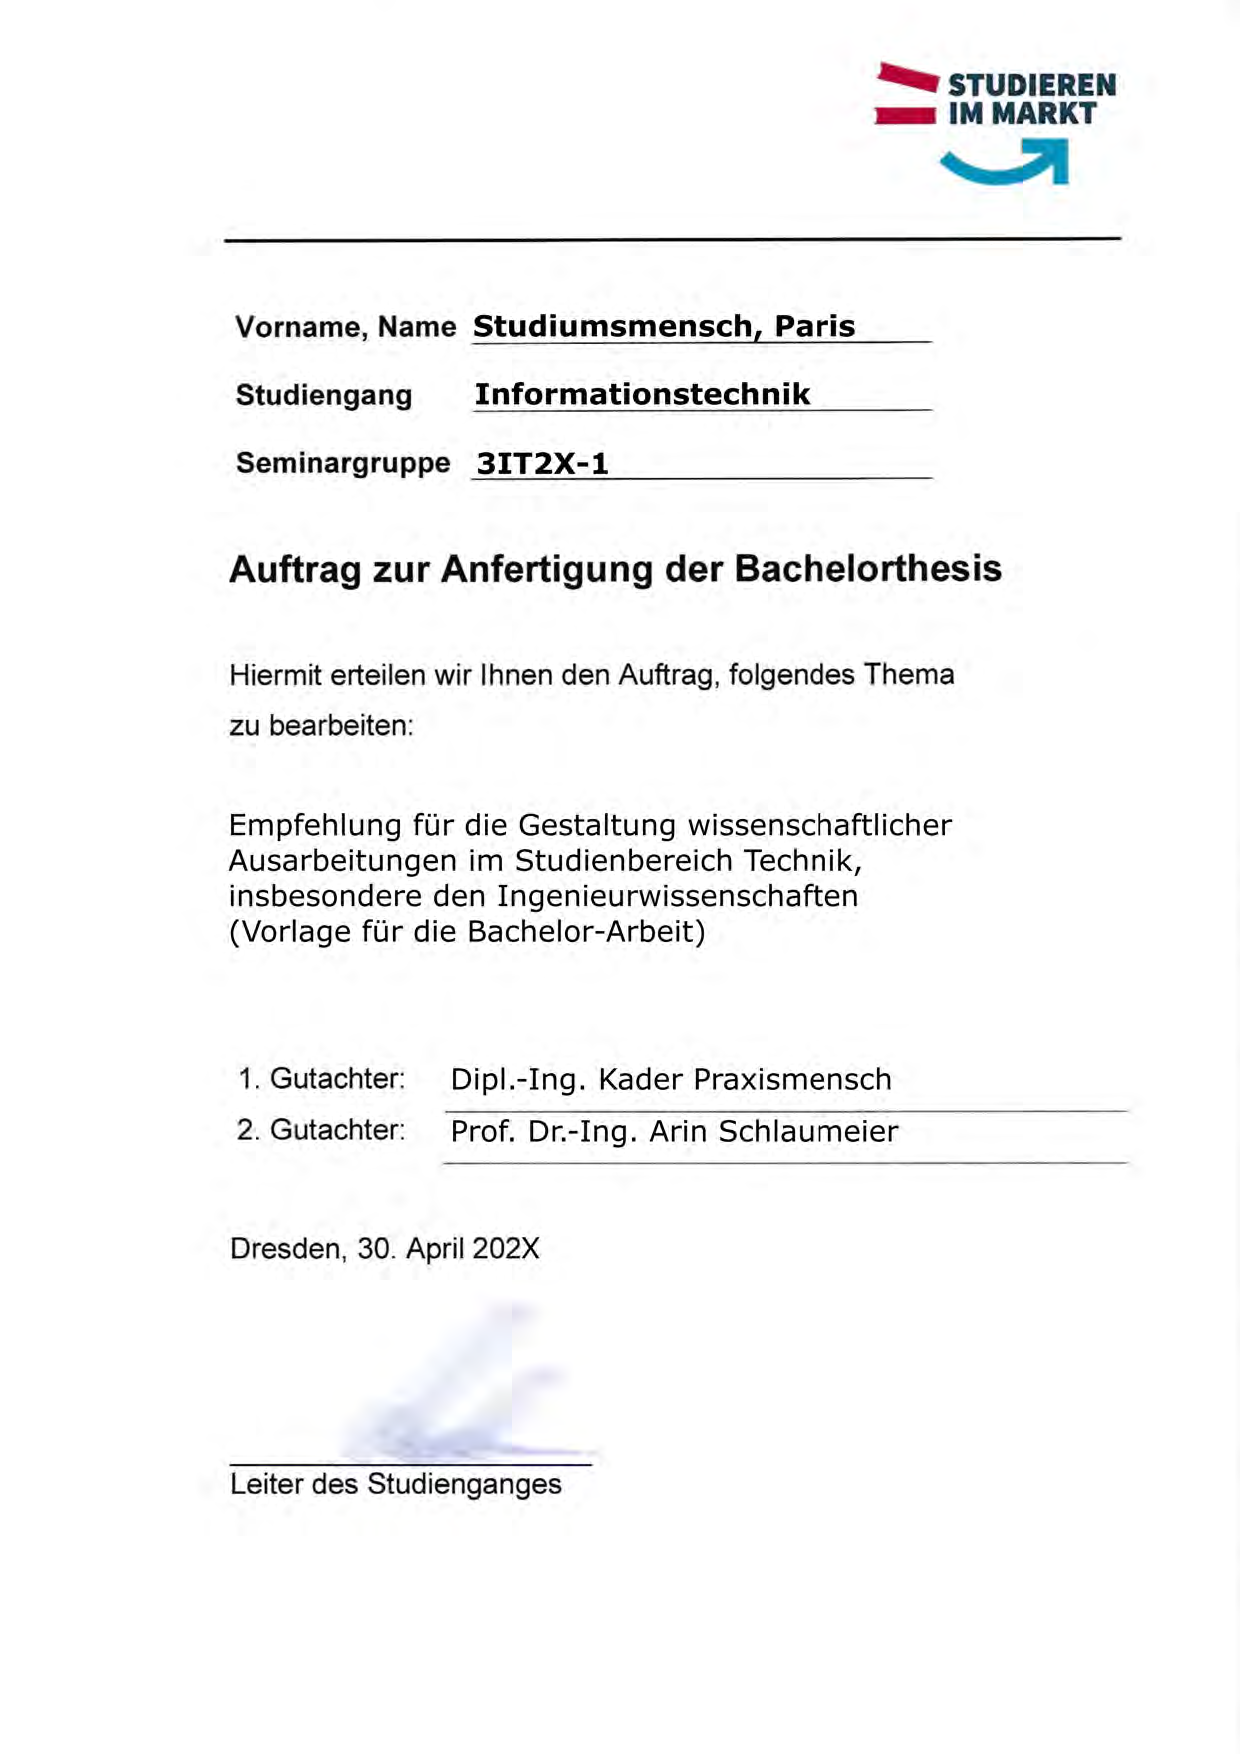
\includepdf[pagecommand={}]{Auftragsblatt.pdf}
}{
    \setcounter{page}{\value{page}+2}
}
\doparttoc
\dopartlof
\dopartlot

\makeatletter
\renewcommand\@pnumwidth{1.25cm}
\makeatother
\cleardoublepage\pdfbookmark{\contentsname}{toc}\tableofcontents\label{refTOC}
\cleardoublepage

\renewcommand{\listtheoremname}{Definitionen, Theoreme \& Beweise}
\cleardoublepage\phantomsection
\renewcommand\thmtformatoptarg[1]{: \enquote{#1}}
\addcontentsline{toc}{chapter}{Definitionen, Theoreme und Beweise}\listoftheorems[numwidth={3.7em},ignoreall,onlynamed={mydef,mytheorem,myproof}]

\renewcommand{\listfigurename}{Abbildungen}
\cleardoublepage\phantomsection
\makeatletter
	\let\org@dottedtocline\@dottedtocline
	\begingroup
		\renewcommand*\@dottedtocline[3]{\org@dottedtocline{#1}{#2}{3.7em}}
		\addcontentsline{toc}{chapter}{Abbildungsverzeichnis}\listoffigures
	\endgroup
	\renewcommand*\@dottedtocline[3]{\org@dottedtocline{#1}{#2}{#3}}
\makeatother

\renewcommand{\listtablename}{Tabellen}
\cleardoublepage\phantomsection
\makeatletter
	\begingroup
		\renewcommand*\@dottedtocline[3]{\org@dottedtocline{#1}{#2}{3.7em}}
		\addcontentsline{toc}{chapter}{Tabellenverzeichnis}\listoftables
	\endgroup
	\renewcommand*\@dottedtocline[3]{\org@dottedtocline{#1}{#2}{#3}}
\makeatother
\cleardoublepage

\renewcommand{\lstlistlistingname}{Quellkode}
\cleardoublepage\phantomsection
\makeatletter
	\begingroup
		\renewcommand*\@dottedtocline[3]{\org@dottedtocline{#1}{#2}{3.7em}}
		\addcontentsline{toc}{chapter}{Quellkodeverzeichnis}\lstlistoflistings
	\endgroup
	\renewcommand*\@dottedtocline[3]{\org@dottedtocline{#1}{#2}{#3}}
\makeatother

% Glossar
\cleardoublepage\phantomsection
\makeatletter
	\begingroup
		\renewcommand*\@dottedtocline[3]{\org@dottedtocline{#1}{#2}{3.7em}}
		\addcontentsline{toc}{chapter}{Glossar}\printglossary
% Wenn Sie keine Seitenangaben für Rücksprünge haben wollen,
% können diese mit der Option „nonumberlist“ unterdrückt werden:
% \printglossary[nonumberlist]
	\endgroup
	\renewcommand*\@dottedtocline[3]{\org@dottedtocline{#1}{#2}{#3}}
\makeatother

\cleardoublepage

%\mainmatter
\pagenumbering{arabic}
\pagestyle{myfancy}
\part{Thesis}\label{pt:thesis}
\chapter{Einleitung}\label{chap:Intro}
Der Leitfaden der Staatlichen Studienakademie Dresden für Abschlussarbeiten\footnote{\label{fn:Leitfaden}Im Genauen: \enquote{Verbindlicher Leitfaden für die Anfertigung und formale Gestaltung wissenschaftlicher (Haus-)Arbeiten an der der Staatlichen Studienakademie Dresden}} ist für Anforderungen in den Ingenieurwissenschaften stellenweise ungeeignet oder widerspricht grundsätzlich den Gepflogenheiten im Fachgebiet. Diese Vorlage hat das Ziel, Studierenden in den Ingenieurwissenschaften eine für das Fachgebiet passendere Vorlage anzubieten.

Diese Vorlage ist bei Overleaf\footnote{\url{https://www.overleaf.com/read/bfmdxnhntbxp} --\,zuletzt am 8. Februar 2023 erfolgreich abgerufen} und Github\footnote{\url{https://github.com/tchara/StADD-Thesis.git} --\,zuletzt am 8. Februar 2023 erfolgreich abgerufen} öffentlich verfügbar.

\comment{Beachten Sie bitte, dass dieses Dokument eine Empfehlung mit ein paar Leitlinien darstellt.\newline Es handelt sich \textbf{nicht} um eine verbindliche Richtlinie.}

\noindent Allgemein gelten die folgenden Grundsätze bei ingenieurwissenschaftlichen Ausarbeitungen:
\begin{itemize}
    \item{
        Ingenieure wollen Ressourcen sparen. Entsprechend sollten Sie sparsam mit Ihrem Textsatz umgehen. Dies bedeutet insbesondere:
        \begin{itemize}
            \item Doppelseitiges Layout (wenn Sie explizit einseitiges Layout wünschen, müssen Sie in der Datei \texttt{thesis.tex} in Zeile $30$ \enquote{twoside} auskommentieren),
            \item Fußnoten wieder verwenden (entweder \enquote{global} oder pro Kapitel),
            \item vollständige Quellenangaben nur im Literaturverzeichnis (im Hauptteil nur Verweise verwenden) und
            \item Sie als Autor dürfen eigene Inhalte kommentieren, wenn Sie die Lesenden beim Verstehen der Inhalte unterstützen wollen. Machen Sie Kommentare so deutlich kenntlich, dass sie sich eindeutig vom restlichen Fließtext unterscheiden! Siehe Beispiel oben.
            \item Der vorherige Punkt ist von Belang, da Sie sich nicht selbst plagiieren können; eigene Vorarbeiten, etc. können Sie nicht als Quellen verwenden! Um Lesende dennoch auf die Existenz von Vorarbeiten hinzuweisen, können Sie einen Kommentar von der Form \enquote{Ergebnisse aus der vorherigen Studienarbeit} o.\,ä. verwenden.
        \end{itemize}
    }
    \item{
        Quellen gehören in das Literaturverzeichnis am Ende (in dieser Vorlage auf Seite~\pageref{Bibliography}). Dabei führen Sie nur Primärquellen auf; wichtig dabei ist, dass als Quelle nur qualifizieren:
        \begin{itemize}
            \item Werke mit mindestens einer namentlich benannten Autor:in, einem Titel und einem Veröffentlichungsdatum (i.\,d.\,R. reicht das Jahr),
            \item Standarde (DIN, ISO, RFC, $\ldots$) oder
            \item \enquote{Berichte aus erster Hand} (zum Beispiel ein Vernehmungsprotokoll, eine Aussage vor Gericht, eine Zeitungsinterview, et cetera).
        \end{itemize}
    }
    \item{
        Insbesondere im Hauptteil der Ausarbeitung --\,in der Regel aber im gesamten Dokument\,-- referenzieren Sie die Quellen im Fließtext/Lauftext indem Sie auf den zitierten Autor\footnote{Das machen Sie mit dem Zitationsstil \enquote{unsrtnat} und der Anweisung \inlinecode{\textbackslash{}citeauthor\{quelle\}}.} oder die Referenz (z.B.\cite{bentley:1999}\footnote{Das hier ist ein spezieller Zitationsstil (\enquote{baalphadin}) für die Berufsakademie, welcher auf dem alphanummerischen DIN-Stil (\enquote{alphadin}) beruht. Sie können aber auch jeden anderen Stil verwenden, solange Sie eindeutig bleiben und nicht zwischen Stilen hin-und-her wechseln. Eine Liste mit Stilen finden Sie in der Overleaf-Hilfe: \url{https://www.overleaf.com/learn/latex/bibtex_bibliography_styles}}) im Quellenverzeichnis verweisen. {\color{red}In den Ingenieurwissenschaften gehören Quellenangaben auf keinen Fall in  Fußnoten!} Das bemerken Sie allein schon an den üblichen Zitierstilen aller großen Outlets, welche in den Ingenieur- und Naturwissenschaften verwendet werden: ACM, APA, CSE, DIN ISO 690 (Vancouver), IEEE, LNI, Springer, etc.\,pp.
    }
    \item{
        In Fußnoten schreiben Sie ausschließlich weiterführende Informationen.
        \begin{itemize}
            \item Bei URLs geben Sie immer das Datum des letzten erfolgreichen Zugriffs an\footnote{Der Grund dahinter ist, dass es sein kann, dass die von Ihnen verlinkte Webseite zwischenzeitlich gegenteilige Inhalte aufweisen oder komplett vom Netz genommen sein könnte. Durch die Datumsangabe ist es den Begutachtenden möglich, im Internet Archive oder in der Wayback Machine den von Ihnen verwendeten Stand zu reproduzieren.}.
            \item Bei Internet-\enquote{Quellen} verlinken Sie die Hauptseite einmal! Nicht für jede Unterseite eine neue Fußnote anlegen!
        \end{itemize}
    }
    \item{
        Fußnoten setzen Sie einmal. Sollten Sie inhaltlich das gleiche später noch einmal benötigen, so verwenden Sie die gleiche Fußnote wieder, selbst wenn sie mehrere Seiten zurückliegen sollte. Hier als Beispiel die Wiederverwendung der Fußnote mit dem Leitfaden\footnoteref{fn:Leitfaden}\textsuperscript{,}\footnote{Wiederverwendete Fußnoten sind im PDF anklickbar und führen Lesende direkt zur entsprechenden Stelle im Dokument. Sie erstellen sie, indem Sie Ihrer Fußnote ein \inlinecode{{\textbackslash}label} geben und dann später mittels \inlinecode{{\textbackslash}footnoteref} referenzieren.}.
    }
\end{itemize}

\comment{Die in den Wirtschafts- und Geisteswissenschaften weit verbreitete Praxis, Quellen und Referenzen in den Fußnoten aufzuführen hat auch seine guten Gründe und Vorteile. Wenn Sie einzelne Seiten aus einem Werk kopieren sind sofort Primärtext und Quellenangaben auf einem Blatt. Die Kopie ist sofort verwendbar. -- In den Ingenieruwissenschaften müssen Sie zusätzlich zum Primärtext auch das Literaturverzeichnis kopieren damit die Kopie vollständig ist.}

Beachten Sie, dass bei doppelseitigem Druck neue Kapitel immer auf einer rechten Seite beginnen, auch wenn das zu einer leeren linken Seite davor führt.

Beim doppelseitigen Druck ist der innere Rand der Seiten schmaler als der äußere, da nach der Bindung der gemeinsame innere\footnote{Abstand des rechten Randes des Textes der linken Seite zum linken Rand des Textes der rechten Seite} Rand optisch genau so groß sein soll, wie die äußeren Ränder. --\,Bei den hier gewählten Rändern haben Sie außen einen größeren Korrekturrand. Dieser ist notwendig, da der in dieser Vorlage voreingestellte Zeilenabstand den Begutachtenden keine Kommentierung im Fließtext erlaubt.

Wie Sie sicherlich bemerkt haben, ist diese Vorlage so konfiguriert, dass Absätze einen kleinen vertikalen Abstand zueinander haben. Die erste Zeile jedes Absatzes ist \emph{nicht} eingerückt. Dieses Verhalten können Sie in der Datei \texttt{config.tex} anpassen:
\begin{itemize}
    \item \inlinecode{\textbackslash setlength\{\textbackslash parindent\}\{0pt\}} --\,definiert den Zeilenvorschub, hier auf Null, und
    \item \inlinecode{\textbackslash setlength\{\textbackslash parskip\}\{4pt\}} --\,definiert die Absatzdistanz, hier auf 4 Punkte.
\end{itemize}

Die Anweisung \inlinecode{\textbackslash noindent} zu Beginn eines Absatzes unterdrückt den Zeilenvorschub. Das ist von Relevanz, falls Sie einen Wert ungleich Null für das \inlinecode{\textbackslash parindent} definiert haben. Es ist nämlich Standardeinstellung von \LaTeX{}, dass der erste Absatz nach der Überschrift des Kapitels bzw. der Sektion nicht eingerückt wird, alle anderen aber schon. Das ist unschön, wenn Sie ein Blockelement im Fließtext haben, wie zum Beispiel zu Beginn dieses Kapitels nach dem Kommentar. Wie Sie im Quelltext sehen können, ist an der entsprechenden Stelle ein \inlinecode{\textbackslash noindent} platziert. Beobachten Sie das Verhalten, wenn Sie in der \texttt{config.tex} den Wert für \inlinecode{\textbackslash parindent} verändern!

Apropos Absätze: {\color{red}Absatzumbrüche erzeugen Sie in \LaTeX\ immer mit einem doppelten Zeilenumbruch im Quelltext.} Achten Sie also drauf, wo Sie einzelne und doppelte Zeilenumbrüche im Quelltext verwenden. Erzeugen Sie keine Absatzumbrüche durch doppelte \LaTeX{}-Zeilenumbrüche (\inlinecode{\textbackslash\textbackslash\textbackslash\textbackslash}) oder entsprechende Ersatzkommandos wie \texttt{\textbackslash newline}. Überlegen Sie auch genau, wann Sie Seitenumbrüche (\inlinecode{\textbackslash clearpage} und \inlinecode{\textbackslash cleardoublepage}) verwenden.

Gerne verwenden Studierende für wichtige Begriffe einen \Gls{glossar}. Das ist recht einfach und wird in dieser Vorlage mit dem \enquote{\texttt{glossaries}}-Paket umgesetzt. Alle Glossareinträge befinden sich in der Datei \texttt{frontbackmatter\textbackslash Glossary.tex} und sollten dort von Ihnen verwaltet werden. Sie werden mit der Anweisung \inlinecode{\textbackslash Gls\{Eintrag\}} referenziert.

Über das \enquote{glossaries}-Paket können Sie auch \Glspl{abk} definieren. Auf die definierten \Glspl{abk} greifen Sie dann zu mit
\begin{itemize}
    \item \inlinecode{\textbackslash acrshort\{abk\}}: erzeugt nur die Abkürzung, hier also \enquote{\acrshort{abk}},
    \item \inlinecode{\textbackslash acrlong\{abk\}}: erzeugt das Ausgeschriebene, hier also \enquote{\acrlong{abk}}, sowie
    \item \inlinecode{\textbackslash acrfull\{abk\}}: erzeugt beides, hier also \enquote{\acrfull{abk}}.
\end{itemize}

Außerdem gibt es, wie Sie sicherlich gemerkt haben, auch ein paar Tricks für die korrekte Referenzierung des Plurals. Dazu verwenden Sie die Anweisung \inlinecode{\textbackslash Glspl\{abk\}}. Beachten Sie, dass beim erstmaligen Aufruf (siehe oben) das Verhalten von \texttt{acrfull} verwendet wird.

Näheres zum Umgang mit dem \enquote{glossaries}-Paket finden Sie in der Overleaf-Hilfe unter \url{https://www.overleaf.com/learn/latex/Glossaries}.

Ein letzter Stilhinweis: Vermeiden Sie nach Möglichkeit Silben-, Wort-, Satz- und Absatzwaisen. D.h., dass Sie vermeiden eine neue Zeile oder gar eine ansonsten leere Seite mit nur einer Silbe oder einem einzelnen Wort zu beginnen. Versuchen Sie, Seiten mit weniger als $5$ Zeilen zu vermeiden.

Apropos Silben: Bei langen Kompositen und an manchen Zeilenenden tut sich \LaTeX{} sehr schwer mit der Silbentrennung. Sie haben mehrere Optionen, wie Sie dann vorgehen können:
\begin{itemize}
    \item{Zwingen Sie das ganze Wort in die neue Zeile indem Sie eine \texttt{mbox} um das Wort legen. Das ist auch sinnvoll, wenn Sie Gesetze o.\,ä. referenzieren und sie zusammenbehalten wollen: \inlinecode{\textbackslash mbox\{§§ 126, 126a BGB\}}.}
    \item{Sie können \LaTeX{} explizit die Silbenstrennung vorgeben, indem Sie die Trennstellen markieren: \inlinecode{Do\textbackslash-nau\textbackslash-dampf\textbackslash-schiff\textbackslash-fahrt}. Bei häufig verwendeten Wörtern definieren Sie die Silbentrennung lieber am Ende des Vorspanns mit der \texttt{hyphenation}-Umgebung (in dieser Vorlage in der \texttt{thesis.tex} in Zeile $47$). Aber Vorsicht: \LaTeX{} wird die Wörter dann \emph{nur} an diesen Stellen trennen.}
    \item{Nicht zu trennende Wörter können Sie statt mit einer \texttt{mbox} auch mit einer Tilde (geschütztes Leerzeichen) binden: \inlinecode{§§\textasciitilde 126,\textasciitilde 126a\textasciitilde BGB}.}
    \item{Das geschützte halbe Leerzeichen verwenden Sie bei Abkürzungen wie \inlinecode{z.\textbackslash,B.}.}
\end{itemize}

Der Rest dieses Werkes ist lediglich ein Platzhalter für die grundständige Struktur einer ingenieurwissenschaftlichen Ausarbeitung und gibt dabei ein paar Einblicke in den Textsatz mit dieser \LaTeX{}-Vorlage\footnote{Eine Word-Vorlage wurde erst einmal nicht erstellt. Sollten Sie Word bevorzugen, folgen Sie sinngemäß dieser Vorlage!}\textsuperscript{,}\footnote{Im Allgemeinen finden Sie in den Kapiteln Hinweise auf die jeweils geforderten Inhalte.}. Befolgen Sie mit Ausnahme der hier folgenden Hinweise ansonsten den eingangs dieses Kapitels erwähnten  Leitfaden\footnoteref{fn:Leitfaden}.


\section{Motivation}\label{sec:Intro:Motivation}
Beschreiben Sie die Motivation hinter der Themenstellung. Weshalb ist es wichtig, dass Sie das Thema wissenschaftliche bearbeiten und quantitativ belastbare Ergebnisse produzieren?


\section{Ziel der Arbeit}\label{sec:Intro:Goal}
Beschreiben Sie kurz und prägnant das Ziel Ihrer Arbeit. Sollten Sie Thesen haben, wäre hier ein guter Ort, um sie erstmals aufzuführen.

\comment{Beachten Sie unbedingt die Hinweistexte in der \texttt{config.tex}, beispielsweise zum Auftragsblatt (siehe \hyperlink{taskpage}{Seite }\pageref{taskpage}) oder dem Einsatz von Bib\LaTeX\ anstelle von Bib\TeX.}


\section{Gliederung}\label{sec:Intro:Structure}
Beschreiben Sie die Gliederung Ihrer Abschlussarbeit, damit Lesende einen schnellen Überblick über den Inhalt bekommen. Beispiel:

\emph{Der Rest dieser Ausarbeitung ist entsprechend der Mehrheit ingenieurwissenschaftlicher Arbeiten gegliedert. Nach einer Übersicht der notwendigen Grundlagen und der wichtigsten verwandten Arbeiten im nächsten Kapitel folgt ab Seite~\pageref{chap:Concept} die eigene Konzeption eines Lösungsansatzes. Die Umsetzbarkeit dessen wird in \autoref{chap:ProofOfConcept} ab Seite~\pageref{chap:ProofOfConcept} dargestellt. Die auf Basis der prototypischen Umsetzung durchgeführte Evaluation schließt sich ab Seite~\pageref{chap:Evaluation} an. Die Auswertung der Evaluation erfolgt im \autoref{chap:Results} \enquote{\nameref{chap:Results}} bevor die zusammenfassende Diskussion die Ausarbeitung abschließt.}
\chapter{Grundlagen und verwandte Arbeiten}\label{chap:RelatedWork}
Beschreiben Sie in diesem Kapitel die Ergebnisse Ihrer Literaturrecherche.

\section{Grundlagen}\label{sec:RelatedWork:Foundations}
Falls Sie fundamentale Grundlagen beschreiben müssen, fügen Sie diese entsprechend hier vor der Literaturrecherche ein.

\subsection{Mathematische Grundlagen}\label{subsec:RelatedWork:Foundations:Maths}
Sollten Sie auf wichtige mathematische Grundlagen eingehen (beispielsweise weil Ihr toller neuer Kryptografiealgorithmus eine Erweiterung des Chinesischen Restsatzes voraussetzt), fügen Sie diese Grundlagen ebenfalls vor der Literaturrecherche ein.

\subsection{Technische Grundlagen}\label{subsec:RelatedWork:Foundations:Techs}
Technische Grundlagen wie sie beispielsweise in DIN, ISO, etc. beschrieben sind, sollten Sie auch getrennt aufführen.

\section{Verwandte Arbeiten}\label{sec:RelatedWork:Publications}
Der Teil \enquote{Verwandte Arbeiten} (in englischer Literatur i.d.R. \emph{Related Work}) betrachtet alle relevanten wissenschaftlichen Literaturquellen.

\section{Stand der Technik}\label{sec:RelatedWork:SotA}
Von wissenschaftlichen Quellen sollten Sie den Stand der Technik (in englischer Literatur i.\,d.\,R. \emph{State of the Art} oder \emph{SotA}) streng trennen. Hier betrachten Sie existierende Lösungen am Markt, etc.

\subsection{Best Practices}\label{subsec:RelatedWork:BestPractices}
Sollten sich aus der Marktanalyse klare Best Practices ergeben, fassen Sie diese am besten noch einmal separat zusammen.
\chapter{Eigenes Konzept}\label{chap:Concept}
Beschreiben Sie auf Basis der Ergebnisse Ihrer Literaturrecherche Ihr eigenes Konzept. Dazu ist in einem vorherigen Schritt (am Ende von \autoref{chap:RelatedWork}) oder direkt zu Beginn dieses Konzept-Kapitels eine Anforderungsanalyse sinnvoll. Am Ende der Anforderungsanalyse sollte eine Tabelle stehen, in welcher die Anforderungen nach Wichtigkeit gruppiert aufgeführt sind. Die gleiche Tabelle mit zwei zusätzlichen Spalten sollte sich im \autoref{chap:Results} wieder finden. Die beiden zusätzlichen Spalten sollten mit Häckchen ($\surd$) oder Kreuz ($\times$) die Erfüllung der jeweiligen Anforderung aufzeigen und, im $\surd$-Fall die Güte (\enquote{Falls \enquote{Ja}, wie gut?}), im $\times$-Fall die Gründe (\enquote{Falls \enquote{Nein}, weshalb nicht?}), aufführen. Um die Frage \enquote{Falls \enquote{Ja}, wie gut?} beantworten zu können, sollten Sie mit der Anforderungsanalyse auch eine Evaluationsmethodik und die zugehörige Evaluationsmetrik definieren.
\chapter{Implementierung / Proof of Concept}\label{chap:ProofOfConcept}
Nachweis der Umsetzbarkeit Ihres Konzeptes, in der Regel durch eine prototypische Implementierung oder einen Nachweis durch Probandenbefragungen, etc.

Beschreiben Sie die \enquote{Highlights} Ihres Proof-of-Concepts. Der gesamte Quellkode, die Konstruktionspläne Ihres Modells, die vollständigen CAD-basierten Berechnungen, etc. sind als Ganzes uninteressant. Konzentrieren Sie sich auf besonders interessante Probleme und wie Sie sie gelöst haben. Abenteuerliches Beispiel: Sie haben in Ihrem Konzept einen Mechanismus, der das Halteproblem löst. Im Proof-of-Concept haben Sie festgestellt, dass ein NP-harter Isomorphismus ausreicht. Zeigen Sie also die paar Kodezeilen, die diesen Isomporphismus umsetzen. ;-)

\comment{Das Kapitel heißt entweder \enquote{Implementierung} \emph{oder} \enquote{Proof of Concept} --\,Nicht wie o.\,g. beides.}

\comment{Bei der Implementierung von Software sollten Sie sich an \cite{sommerville1992} orientieren!}
\chapter{Evaluation}\label{chap:Evaluation}
Evaluation Ihres Konzeptes entlang der vor der Konzeptionierung festgelegten Evaluationsmetrik. Hier erfolgt insbesondere die Prüfung der Erfüllung aller Anforderungen.

Achten Sie darauf, dass die Evaluation nachvollziehbar ist. Idealerweise fassen Sie Ergebnisse in Tabellen zusammen. Sollten Sie Umfragen und Probandenstudien durchgeführt haben, so können Sie --\,Sie müssen aber nicht\,-- die einzelnen Studienkomponenten in den Anhang (in dieser Vorlage ab Seite~\pageref{apdx:A}) legen.

\comment{
    Sollten Sie Performance-Metriken o.ä. erfasst haben, bei denen die Vergleichbarkeit unbedingt gegeben sein muss, ist die Angabe von Hardware-Spezifikationen in der Regel notwendig.
}

\noindent Für Performance-Tests wurde ein System mit den folgenden Spezifikationen verwendet:
\begin{itemize}
    \item AMD Ryzen 9 5900X,
    \item Corsair Vengence LPX Black DDR4-3600 32GB,
    \item MSI GeForce GTX 1660 Ti Gaming X 6G
    \item MSI MPG X570 Gaming Plus, sowie
    \item Samsung 970 Evo Plus (NVMe) 500GB.
\end{itemize}
\chapter{Ergebnisse}\label{chap:Results}
Hier sollten Sie einerseits explizit Ihre Forschungsfragen beantworten, andererseits näher die Ergebnisse beleuchten. Falls eine Frage mit \enquote{Ja} beantwortet wurde, dann sollten Sie direkt die Frage \enquote{Wie gut?} beantworten. Falls eine Frage mit \enquote{Nein} beantwortet wurde, dann sollten Sie direkt die Frage \enquote{Weshalb nicht?} beantworten.

Sollten Sie anstatt mit Forschungsfragen mit Hypothesen in die Arbeit gegangen sein, sollten Sie spätestens hier die Bestätigung oder die Widerlegung führen. Im Falle einer Bestätigung ist wieder die Frage \enquote{Wie gut?} zu beantworten. Im Falle einer Widerlegung ist eine Antithese aufzustellen, welche mit etwas zusätzlicher Untersuchung (zweite Evaluation) zu einer Synthese führen sollte. Ansonsten im letzten Abschnitt des letzten Kapitels (Zusammenfassung $rarr$ Ausblick) als zukündtige Fortsetzungsmöglichkeit aufführen.
\chapter{Zusammenfassung und Ausblick}\label{chap:Conclusion}
Um die Arbeit abzurunden sollten Sie noch einmal in eine aussagekräftige Zusammenfassung investieren. Diese schließen Sie ab mit einer Betrachtung der offen gebliebenen Aspekte der Ausarbeitung sowie zukünftigen Fortsetzungsmöglichkeiten.

\section{Zusammenfassung}\label{sec:Conclusion:Summary}
In dieser Sektion fassen Sie die wichtigsten Forschungsergebnisse noch einmal zusammen. 

\section{Ausblick}\label{sec:Conclusion:FutureWork}
Offene Aspekte und/oder zukünftige Fortsetzungsmöglichkeiten sollten Sie aufzeigen und --\,wenn Sie über das Erwartungsmaß hinaus Ihre Kenntnisse demonstrieren wollen\,-- eine Abschätzung des notwendigen Aufwandes (Personenstunden; Bachelor-, Master- oder Diplomarbeit; etc.) abgeben.

%
% Das folgende Label ist für die korrekte Zählung der Seitenzahl im
% Autorenreferat zwingend an dieser Stelle erforderlich.
% Stellen Sie sicher, dass es am Ende dieses Kapitels steht!
\label{contentPages:End}
%*************************************************************************
% Literaturverzeichnis
%*************************************************************************
\cleardoublepage
\renewcommand{\bibname}{Quellenverzeichnis}
\bibliographystyle{baalphadin}

\pdfbookmark[-1]{Quellenverzeichnis}{pdf-Bibliography}%
\phantomsection%
\addcontentsline{toc}{chapter}{Quellenverzeichnis}%
% BibTeX:
\bibliography{bibliography}\label{Bibliography}
% BibLateX:
% \printbibliography


\clearpage\section*{Hilfsmittel}\label{Tools}
Zur Erstellung der vorliegenden Abschlussarbeit wurden die folgenden Hilfsmittel verwendet:
% Seien Sie so spezifisch wie möglich!
\begin{itemize}
	\item ChatGPT --\,\url{https://chat.openai.com/chat},
	\item Comprehensive \TeX Archive Network, The --\,\url{http://ctan.org},
	\item dict.leo.org by LEO GmbH,
	\item Encyclop{\ae}dia Britannica,
	\item Gemeinsame Bibliothek der BA Dresden und der ehs Dresden,
	\item Google-Scholar --\,\url{https://scholar.google.com},
	\item Korrekturlesende (namentlich: Erika und Franz Mustermensch),
	\item Microsoft Office 365 University (2301 Build 16026.20200, x64),
	\item Microsoft Visio Professional 2019 (2301 Build 16026.20200, x64),
	\item Microsoft Windows 11 (22H2 Build 22621.1265, x64),
	\item Notepad++ 8.4.8 (32 Bit),
	\item Overleaf --\,\url{https://www.overleaf.com},
	\item Paint.NET (5.0.1, x86),
	\item S{\"a}chsische Landesbibliothek \mbox{--\,Staats}- und Universit{\"a}tsbibliothek Dresden, und
	\item Wiktionary.
\end{itemize}

\comment{
    Sie sollten bei Software eine möglichst abschließende und präzise Liste (inkl. Versionsnummer, etc.) angeben.}

\comment{
    Seien Sie bei Hardware so präzise wie möglich, wenn die Hardware Einfluss auf Messergebnisse o.\,ä. hat. Angaben zum Setup Ihrer Versuchsumgebung geben Sie bei der Beschreibung der Methodik (siehe \hyperref[comment:Setup]{Kommentar} in \autoref{chap:Evaluation}), nicht auf einer gesonderten Seite wie hier!
}
\comment{
    Sollte die verwendete Software Einfluss auf Ihre Messergebnisse haben, z.\,B. wenn Sie Usability-Tests unter Windows und MacOS durchführen, geben Sie die entsprechenden Informationen ebenfalls bei der Beschreibung der Methodik an (siehe \hyperref[comment:Setup]{Kommentar} in \autoref{chap:Evaluation}). --\,Die Liste auf dieser Seite beschränkt sich auf die Erstellung der Abschlussarbeit als Schriftwerk, nicht auf ihre wissenschaftlichen Inhalte.
}
%*************************************************************************
% Anhang
%*************************************************************************
%\backmatter
\appendix
\cleardoublepage
\pagenumbering{Roman}
\part{Anhang}
\chapter{Appendix Test}\label{apdx:A}
\section{Tabellen}\label{sec:apdx:Tables}
\begin{table}[hbt]
	\begin{center}
		\begin{tabular}{l|cc|cc|cc|cc}
			&
			\multicolumn{2}{c|}{\small\textbf{2013/06}} &
			\multicolumn{2}{c|}{\small\textbf{2014/06}} &
			\multicolumn{2}{c|}{\small\textbf{2015/04}} &
			\multicolumn{2}{c}{\small\textbf{2015/06}} \\

			{\small\textbf{Parameter}} &
			{\small\textbf{$\overline{X}^{13|6}$}} &
			{\small\textbf{$\sigma_X^{13|6}$}} &
			{\small\textbf{$\overline{X}^{14|6}$}} &
			{\small\textbf{$\sigma_X^{14|6}$}} &
			{\small\textbf{$\overline{X}^{15|4}$}} &
			{\small\textbf{$\sigma_X^{15|4}$}} &
			{\small\textbf{$\overline{X}^{15|5}$}} &
			{\small\textbf{$\sigma_X^{15|6}$}} \\
            \midrule

			{Alter} &
			$20.6$ & $2.26$ &
			$20.5$ & $2.23$ &
			$20.6$ & $2.27$ &
			$20.4$ & $2.29$ \\

			{Geschlecht$^{\ast}$} &
			$.93$ & n/a &
			$.92$ & n/a &
			$.88$ & n/a &
			$.86$ & n/a \\

			{Zugehörigkeit$^{\oplus}$} &
			$.06$ & n/a &
			$.03$ & n/a &
			$.02$ & n/a &
			$.01$ & n/a \\

			{Durchgang$^{\mp}$} &
			$1.16$ & $.42$ &
			$1.14$ & $.37$ &
			$1.21$ & $.48$ &
			$1.19$ & $.44$ \\

			{Pflichtmodul$^{\bigtriangledown}$} &
			$.36$ & n/a &
			$.33$ & n/a &
			$.31$ & n/a &
			$.31$ & n/a \\

			{Prüfung$^{\bigtriangledown}$} &
			$.32$ & n/a &
			$.29$ & n/a &
			$.30$ & n/a &
			$.26$ & n/a \\

			{Interesse$^{\bigtriangledown}$} &
			$.75$ & n/a &
			$.78$ & n/a &
			$.73$ & n/a &
			$.72$ & n/a \\
			
			\midrule
			\multicolumn{4}{l}{$\ast$: $0$\ldots weiblich, $1$\ldots männlich} &
			\multicolumn{5}{r}{$\oplus$: $0$\ldots TU~Dresden, $1$\ldots abdere} \\
			\multicolumn{6}{l}{$\mp$: $1$\ldots Erster, $2$\ldots Zweiter, $3$\ldots Dritter oder mehr} &
			\multicolumn{3}{r}{$\bigtriangledown$: $0$\ldots ja, $1$\ldots nein}
		\end{tabular}
	\end{center}
	\vspace{-1em}
	\caption[Komposition der Studierendengruppe]{Komposition der Studierendengruppe im betrachteten Setup}\label{tab:Students}
\end{table}

\lipsum[10]

\begin{mytable}
	\begin{center}
		\begin{longtable}{c|p{1.7cm}|ccccc|cc|cc|c}
			\multicolumn{2}{c|}{} & \multicolumn{5}{c|}{\textbf{Diagramm}} & \multicolumn{2}{c|}{\textbf{Prüfung \&}} & \multicolumn{2}{c|}{} & \\
			\multicolumn{2}{c|}{} & \multicolumn{3}{c}{\textbf{UML}} & \multicolumn{2}{c|}{\textbf{andere}} & \multicolumn{2}{c|}{\textbf{Unterstützung}} & \multicolumn{2}{c|}{\textbf{Analyse}} & \\
			{\rotatebox{90}{\parbox{1.5cm}{\textbf{Übung}}}} & \textbf{Aufgaben\-thema} & {\rotatebox{90}{\parbox{1.5cm}{\raggedright\small\textbf{Topologie}}}} & {\rotatebox{90}{\parbox{1.5cm}{\raggedright\small\textbf{Sequenz}}}} & {\rotatebox{90}{\parbox{1.5cm}{\raggedright\small\textbf{Zustand}}}} & {\rotatebox{90}{\parbox{1.5cm}{\raggedright\small\textbf{Schema}}}} & {\rotatebox{90}{\parbox{1.5cm}{\raggedright\small\textbf{Graph}}}} & {\rotatebox{90}{\parbox{1.5cm}{\raggedright\small\textbf{Formel}}}} & {\rotatebox{90}{\parbox{1.5cm}{\raggedright\small\textbf{Tabelle}}}} & {\rotatebox{90}{\parbox{1.5cm}{\raggedright\small\textbf{DIY-\newline Beispiel}}}} & {\rotatebox{90}{\parbox{1.5cm}{\raggedright\small\textbf{Wireshark-Trace}}}} & {\rotatebox{90}{\parbox{1.5cm}{\raggedright\small\textbf{Prosa}}}} \\
			\toprule
			\endfirsthead

			\multicolumn{12}{l}{{$\leadsto$\,fortgesetzt von vorheriger Seite.}} \\
			\toprule
			\multicolumn{2}{c|}{} & \multicolumn{5}{c|}{\textbf{Diagramm}} & \multicolumn{2}{c|}{\textbf{Prüfung \&}} & \multicolumn{2}{c|}{} & \\
			\multicolumn{2}{c|}{} & \multicolumn{3}{c}{\textbf{UML}} & \multicolumn{2}{c|}{\textbf{andere}} & \multicolumn{2}{c|}{\textbf{Unterstützung}} & \multicolumn{2}{c|}{\textbf{Analyse}} & \\
			{\rotatebox{90}{\parbox{1.5cm}{\textbf{Übung}}}} & \textbf{Aufgaben\-thema} & {\rotatebox{90}{\parbox{1.5cm}{\raggedright\small\textbf{Topologie}}}} & {\rotatebox{90}{\parbox{1.5cm}{\raggedright\small\textbf{Sequenz}}}} & {\rotatebox{90}{\parbox{1.5cm}{\raggedright\small\textbf{Zustand}}}} & {\rotatebox{90}{\parbox{1.5cm}{\raggedright\small\textbf{Schema}}}} & {\rotatebox{90}{\parbox{1.5cm}{\raggedright\small\textbf{Graph}}}} & {\rotatebox{90}{\parbox{1.5cm}{\raggedright\small\textbf{Formel}}}} & {\rotatebox{90}{\parbox{1.5cm}{\raggedright\small\textbf{Tabelle}}}} & {\rotatebox{90}{\parbox{1.5cm}{\raggedright\small\textbf{DIY-\newline Beispiel}}}} & {\rotatebox{90}{\parbox{1.5cm}{\raggedright\small\textbf{Wireshark-Trace}}}} & {\rotatebox{90}{\parbox{1.5cm}{\raggedright\small\textbf{Prosa}}}} \\
			\toprule
			\endhead

			\bottomrule
			\multicolumn{12}{r}{Fortsetzung auf nächster Seite\,$\leadsto$} \\
			\endfoot

			\multicolumn{12}{c}{\tiny} \\
			\caption[Mehrseitige Tabelle]{Beispiel für eine mehrseitige Tabelle mit \enquote{longtable}-Umgebung.}\label{tab:TopicsRN}
			\endlastfoot

			\multirow{4}{*}{\rotatebox{90}{$\leftarrow$~U01}} & {\raggedright Computer\-netzwerk\-strukturen} & $\bullet$ & & & & & $\bullet$ & $\bullet$ & & & \\
			\cline{2-12}
			& {\raggedright Dienste und Protokolle} & & $\bullet$ & & $\bullet$ & & & $\bullet$ & & & $\bullet$ \\
			\cline{2-12}
			& {\raggedright Dienst\-elemente} & & $\bullet$ & $\bullet$ & & & & $\bullet$ & & & \\
			\cline{2-12}
			& {\raggedright OSI-Referenz\-modell} & & $\bullet$ & & $\bullet$ & & $\bullet$ & & & & \\
			\midrule

			\multirow{5}{*}{\rotatebox{90}{$\leftarrow$~U02}} & {\raggedright Nyquist-Theorem} & & & & & & $\bullet$ & & & & \\
			\cline{2-12}
			& {\raggedright PCM} & & & & $\bullet$ & & $\bullet$ & & & & \\
			\cline{2-12}
			& {\raggedright Modulation} & & & & $\bullet$ & & & $\bullet$ & & & \\
			\cline{2-12}
			& {\raggedright Line-Encoding} & & & & $\bullet$ & & $\bullet$ & & & & $\bullet$ \\
			\cline{2-12}
			& {\raggedright Multiplexing} & & & & & & $\bullet$ & $\bullet$ & & & $\bullet$ \\
			\midrule

			\multirow{4}{*}{\rotatebox{90}{$\leftarrow$~U03}} & {\raggedright Ethernet} & $\bullet$ & $\bullet$ & & $\bullet$ & & $\bullet$ & & & & \\
			\cline{2-12}
			& {\raggedright Switches} & $\bullet$ & & & & & $\bullet$ & & & & \\
			\cline{2-12}
			& {\raggedright transparente Bridges} & $\bullet$ & & & $\bullet$ & & & & & & $\bullet$ \\
			\cline{2-12}
			& {\raggedright Wireless-LAN} & & & & & & $\bullet$ & & & & \\
			\midrule

			\multirow{6}{*}{\rotatebox{90}{$\leftarrow$~U04}} & {\raggedright WiMAX} & & & & & & & $\bullet$ & & & $\bullet$ \\
			\cline{2-12}
			& {\raggedright RPR} & $\bullet$ & & & & & & & & & \\
			\cline{2-12}
			& {\raggedright Carrier-Ethernet} & $\bullet$ & & & $\bullet$ & & & & & & $\bullet$ \\
			\cline{2-12}
			& {\raggedright MPLS} & $\bullet$ & & & $\bullet$ & & & $\bullet$ & & & \\
			\cline{2-12}
			& {\raggedright SONET, SDH, OTN} & & & & $\bullet$ & & $\bullet$ & & & & \\
			\cline{2-12}
			& {\raggedright VPN} & $\bullet$ & & $\bullet$ & & & & & $\bullet$ & & $\bullet$ \\
			\midrule

			\multirow{5}{*}{\rotatebox{90}{$\leftarrow$~U05}} & {\raggedright Rahmen\-bildung} & & & & $\bullet$ & & & $\bullet$ & & & $\bullet$ \\
			\cline{2-12}
			& {\raggedright ECC} & & & & $\bullet$ & & $\bullet$ & $\bullet$ & & & \\
			\cline{2-12}
			& {\raggedright Paritäts\-bit} & & & & $\bullet$ & & & $\bullet$ & & & \\
			\cline{2-12}
			& {\raggedright CRC} & & $\bullet$ & & & & $\bullet$ & & & & \\
			\cline{2-12}
			& {\raggedright Stop-and-Wait-Protokoll} & & $\bullet$ & & $\bullet$ & & & & & & $\bullet$ \\
			\midrule

			\multirow{5}{*}{\rotatebox{90}{$\leftarrow$~U06}} & {\raggedright OSPF} & $\bullet$ & & & & $\bullet$ & $\bullet$ & $\bullet$ & & & \\
			\cline{2-12}
			& {\raggedright IP-Pakete} & & & & $\bullet$ & & & & & $\bullet$ & $\bullet$ \\
			\cline{2-12}
			& {\raggedright IP:\newline Adressen \& Subnetze} & $\bullet$ & & & $\bullet$ & & $\bullet$ & & & & \\
			\cline{2-12}
			& {\raggedright Routing} & $\bullet$ & $\bullet$ & & $\bullet$ & & & $\bullet$ & & & \\
			\cline{2-12}
			& {\raggedright Überlast\-kontrolle} & & $\bullet$ & & $\bullet$ & & & & & & $\bullet$ \\
			\midrule

			\multirow{4}{*}{\rotatebox{90}{$\leftarrow$~U07}} & {\raggedright Dienste: QoS} & & $\bullet$ & & & & & & & & \\
			\cline{2-12}
			& {\raggedright Schiebe\-fenster\-protokoll} & & $\bullet$ & & $\bullet$ & & & $\bullet$ & & & \\
			\cline{2-12}
			& {\raggedright TCP} & & $\bullet$ & $\bullet$ & & & & $\bullet$ & & $\bullet$ & \\
			\cline{2-12}
			& {\raggedright Protokoll\-vergleich} & & & & & & & $\bullet$ & & & \\
			\midrule

			\multirow{5}{*}{\rotatebox{90}{$\leftarrow$~U08}} & {\raggedright Ethernet-Performance} & & & & $\bullet$ & & $\bullet$ & $\bullet$ & & & \\
			\cline{2-12}
			& {\raggedright Fairness} & & $\bullet$ & & & & & & & & $\bullet$ \\
			\cline{2-12}
			& {\raggedright Überlast\-kontrolle} & & & & $\bullet$ & & $\bullet$ & $\bullet$ & & & \\
			\cline{2-12}
			& {\raggedright Performance-Steigerung} & & & & $\bullet$ & & $\bullet$ & & & & \\
			\cline{2-12}
			& {\raggedright DTN} & $\bullet$ & & & $\bullet$ & & & & & & \\
			\midrule

			\multirow{5}{*}{\rotatebox{90}{$\leftarrow$~U09}} & {\raggedright DNS} & $\bullet$ & & & $\bullet$ & & & $\bullet$ & & & $\bullet$ \\
			\cline{2-12}
			& {\raggedright E-Mail} & & & & & & & & & & $\bullet$ \\
			\cline{2-12}
			& {\raggedright WWW} & & & & $\bullet$ & & & & & $\bullet$ & $\bullet$ \\
			\cline{2-12}
			& {\raggedright SNMP} & & $\bullet$ & & & & & $\bullet$ & & & \\
			\cline{2-12}
			& {\raggedright Zusammen\-spiel von UDP, TCP, HTTP und DNS} & & $\bullet$ & & $\bullet$ & & & $\bullet$ & & & \\
			\midrule

			\multirow{5}{*}{\rotatebox{90}{$\leftarrow$~U10}} & {\raggedright Kodierung} & & & & $\bullet$ & & $\bullet$ & $\bullet$ & & & \\
			\cline{2-12}
			& {\raggedright VoIP} & $\bullet$ & & & $\bullet$ & & & $\bullet$ & & & $\bullet$ \\
			\cline{2-12}
			& {\raggedright RTP} & & & & $\bullet$ & & & & & $\bullet$ & \\
			\cline{2-12}
			& {\raggedright VoIP-Codecs} & & $\bullet$ & & $\bullet$ & & $\bullet$ & & & & \\
			\cline{2-12}
			& {\raggedright Video\-konferenz\-systeme} & $\bullet$ & & & & & $\bullet$ & & & & \\
			\midrule

			\multirow{4}{*}{\rotatebox{90}{$\leftarrow$~U11}} & {\raggedright RPC} & $\bullet$ & $\bullet$ & & & & & & & & $\bullet$ \\
			\cline{2-12}
			& {\raggedright verteilte Transaktionen} & $\bullet$ & $\bullet$ & $\bullet$ & & & & & & & $\bullet$ \\
			\cline{2-12}
			& {\raggedright Web-Services} & & & & & & & & & $\bullet$ & $\bullet$ \\
			\cline{2-12}
			& {\raggedright WebDAV} & & $\bullet$ & & & & & & & $\bullet$ & \\
			\midrule

			\multirow{3}{*}{\rotatebox{90}{$\leftarrow$~U12}} & {\raggedright mobile Kommuni\-kations\-netzwerke} & & & & $\bullet$ & & & & & & $\bullet$ \\
			\cline{2-12}
			& {\raggedright DHCP} & & $\bullet$ & $\bullet$ & & & & $\bullet$ & & & $\bullet$ \\
			\cline{2-12}
			& {\raggedright Mobile-IP} & $\bullet$ & $\bullet$ & & $\bullet$ & & & $\bullet$ & & & \\
			\midrule
			\multicolumn{2}{r|}{Summe} & $18$ & $20$ & $5$ & $32$ & $1$ & $20$ & $24$ & $1$ & $6$ & $21$ \\
			\multicolumn{2}{r|}{Anteil} & $.327$ & $.364$ & $.091$ & $.582$ & $.018$ & $.364$ & $.436$ & $.018$ & $.109$ & $.382$ \\
			\cline{3-7}
			\multicolumn{2}{c}{} & \multicolumn{5}{c}{$76$ Diagramme,} &
 \multicolumn{5}{c}{} \\
			\multicolumn{2}{c}{} & \multicolumn{5}{c}{davon $43$ UML ($56.6\%$)} &
 \multicolumn{5}{c}{} \\
		\end{longtable}
	\end{center}
	\vspace{-1.5em}
\end{mytable}


\begin{mytable}\begin{sidewaystable}
	\begin{center}
		\begin{tabular}{cc|cc|cc|cc|cc|cc|cc|cc|cc}
			\multicolumn{2}{c|}{} &
			\multicolumn{2}{c|}{\rotatebox[origin=c]{270}{\parbox{1.3cm}{\raggedright\small\textbf{before first reading}}}} &
			\multicolumn{2}{c|}{\rotatebox[origin=c]{270}{\parbox{1.3cm}{\raggedright\small\textbf{after first reading}}}} &
			\multicolumn{2}{c|}{\rotatebox[origin=c]{270}{\parbox{1.3cm}{\raggedright\small\textbf{current reading}}}} &
			\multicolumn{2}{c|}{\rotatebox[origin=c]{270}{\parbox{1.3cm}{\raggedright\small\textbf{before first tutorial}}}} &
			\multicolumn{2}{c|}{\rotatebox[origin=c]{270}{\parbox{1.3cm}{\raggedright\small\textbf{after first tutorial}}}} &
			\multicolumn{2}{c|}{\rotatebox[origin=c]{270}{\parbox{1.3cm}{\raggedright\small\textbf{current tutorial}}}} &
			\multicolumn{2}{c|}{\rotatebox[origin=c]{270}{\parbox{1.3cm}{\raggedright\small\textbf{reading \mbox{$\downarrow\bigtriangledown$\hspace*{.35cm}} tutorial}}}} &
			\multicolumn{2}{c}{\rotatebox[origin=c]{270}{\parbox{1.3cm}{\raggedright\small\textbf{tutorial \mbox{$\downarrow\bigtriangledown$\hspace*{.35cm}} reading}}}} \\

			\multicolumn{2}{c|}{data source} &
			{\small\textbf{$\overline{X}$}} &
			{\small\textbf{$\sigma_X$}} &
			{\small\textbf{$\overline{X}$}} &
			{\small\textbf{$\sigma_X$}} &
			{\small\textbf{$\overline{X}$}} &
			{\small\textbf{$\sigma_X$}} &
			{\small\textbf{$\overline{X}$}} &
			{\small\textbf{$\sigma_X$}} &
			{\small\textbf{$\overline{X}$}} &
			{\small\textbf{$\sigma_X$}} &
			{\small\textbf{$\overline{X}$}} &
			{\small\textbf{$\sigma_X$}} &
			{\small\textbf{$\overline{X}$}} &
			{\small\textbf{$\sigma_X$}} &
			{\small\textbf{$\overline{X}$}} &
			{\small\textbf{$\sigma_X$}} \\
			\midrule

			\multirow{3}{*}{15-G1}
			& 15-A1 & $6.38$ & $2.09$ & $5.55$ & $2.13$ & $5.99$ & $2.09$ & $6.39$ & $1.99$ & $6.02$ & $1.98$ & $6.05$ & $2.65$ & $1.89$ & $.62$ & $2.33$ & $.67$ \\
			& 15-A2 & \multicolumn{2}{c|}{not asked} & \multicolumn{2}{c|}{not asked} & 5.97 & 2.21 & \multicolumn{2}{c|}{not asked} & \multicolumn{2}{c|}{not asked} & $6.22$ & $2.25$ & $1.88$ & $.64$ & $2.36$ & $.71$ \\
			& 15-A3 & \multicolumn{2}{c|}{not asked} & \multicolumn{2}{c|}{not asked} & 5.91 & 2.08 & \multicolumn{2}{c|}{not asked} & \multicolumn{2}{c|}{not asked}& $6.27$ & $2.34$ & $1.86$ & $.69$ & $2.44$ & $.76$ \\

			\midrule
			\multirow{3}{*}{15-G2}
			& 15-A1 & $6.24$ & $2.37$ & $5.44$ & $2.20$ & $6.02$ & $2.31$ & $6.12$ & $2.04$ & $6.14$ & $2.14$ & $6.13$ & $1.98$ & $1.88$ & $.59$ & $2.31$ & $.70$ \\
			& 15-A2 & \multicolumn{2}{c|}{not asked} & \multicolumn{2}{c|}{not asked} & 5.98 & 2.16 & \multicolumn{2}{c|}{not asked} & \multicolumn{2}{c|}{not asked} & $6.20$ & $1.97$ & $1.86$ & $.61$ & $2.33$ & $.71$ \\
			& 15-A3 & \multicolumn{2}{c|}{not asked} & \multicolumn{2}{c|}{not asked} & 5.93 & 1.98 & \multicolumn{2}{c|}{not asked} & \multicolumn{2}{c|}{not asked}& $6.30$ & $2.00$ & $1.84$ & $.60$ & $2.37$ & $.77$ \\

			\midrule
			\multirow{3}{*}{15-G3}
			& 15-A1 & $6.29$ & $2.02$ & $5.22$ & $2.10$ & $5.91$ & $2.06$ & $6.42$ & $2.08$ & $5.89$ & $2.51$ & $6.01$ & $2.00$ & $1.88$ & $.59$ & $2.42$ & $.79$ \\
			& 15-A2 & \multicolumn{2}{c|}{not asked} & \multicolumn{2}{c|}{not asked} & 5.93 & 2.27 & \multicolumn{2}{c|}{not asked} & \multicolumn{2}{c|}{not asked} & $6.01$ & $1.99$ & $1.87$ & $.66$ & $2.34$ & $.74$ \\
			& 15-A3 & \multicolumn{2}{c|}{not asked} & \multicolumn{2}{c|}{not asked} & 5.90 & 2.15 & \multicolumn{2}{c|}{not asked} & \multicolumn{2}{c|}{not asked}& $6.00$ & $2.11$ & $1.84$ & $.72$ & $2.37$ & $.76$ \\

			\midrule
			15-CG & $\ast$ & \multicolumn{16}{c}{insufficient data (pool size $9$)} \\

			\midrule
			\multicolumn{18}{l}{$\bigtriangledown$: $1$\ldots yes, $2$\ldots neither, $3$\ldots no} \\

		\end{tabular}
		\caption[Seitwärtstabelle]{mit der \enquote{sidewaystable}-Umgebung drehen Sie Tabellen so, dass sie \enquote{nach außen} zeigen. --\,Die Zellen in der Titelzeile müssen Sie ggf. für linke Seiten ($90^{\circ}$ und \textbackslash{}raggedleft) und --\,wie hier\,-- rechte Seiten ($270^{\circ}$ und \textbackslash{}raggedright) anpassen.}\label{tab:Motivation2015}
	\end{center}
\end{sidewaystable}\end{mytable}



\section{Listen}\label{sec:apdx:Lists}
\noindent Mehrere Listentypen werden von dieser Vorlage unterstützt...

Punkt-Listen sind unsortierte Listen für Auflistungen mit
\begin{itemize}
    \item Punkten,    
    \item[--] kurzen Strichen,
    \item[$-$] langen Strichen,
    \item[$\ast$] Sternchen oder
    \item[$\blacksquare$] sonstigen Markern;
    \item{
        das geht auch in mehrere Ebenen 
        \begin{itemize}
            \item mit automatisch gesetzten Markern oder
            \item[$\alpha$] auch händisch definierten.
        \end{itemize}
    }
\end{itemize}

Sortierte Listen sind in der Regel Aufzählungen sortiert anhand
\begin{enumerate}
    \item arabischer Zahlen,
    \item[II.] römischer Zahlen oder
    % hier von Hand gesetzt, damit die unterschiedlichen Stile
    % im Dokument ohne Hacks direkt beieinander stehen können...
    \item[C.] Buchstaben;
    \setcounter{enumi}{3}
    \item{
        auch sie sind geschachtelt möglich, bspw.
        \begin{enumerate}
            \item Hund,
            \item Katze und
            \item Maus.
        \end{enumerate}
    }
\end{enumerate}

Beachten Sie, dass auch Listen immer vollständige Sätze mit Satzzeichen sein sollten. Das heißt, es gehört ein Komma hinter jedes Element bis auf die letzten beiden. Im vorletzten Element verwenden Sie eine Konjuktion\footnote{\enquote{und}, \enquote{sowie}, etc.pp.} oder eine Disjunktion\footnote{\enquote{oder}, \enquote{aber nicht}, etc.pp.}, sowie im letzten Element einen Punkt.

Mehr zu Listen und ihren Möglichkeiten finden Sie in der Overleaf-Hilfe:
\begin{center}
    \url{https://www.overleaf.com/learn/latex/Lists}
\end{center}

Manchmal wird es sehr hässlich, wenn Sie viele kurze Listenelemente haben. Das führt dazu, dass Sie einen \enquote{langen Schlauch} mit viel Whitespace rechts davon erhalten. Dann bietet es sich an, die Listen mehrspaltig setzen zu lassen:
\begin{multicols}{3}
\begin{itemize}
    \item erstes Element,
    \item zweites Element,
    \item drittes Element,
    \item viertes Element,
    \item fünftes Element,
    \item sechstes Element,
    \item siebtes Element,
    \item achtes Element sowie
    \item neuntes Element,
    \item zehntes Element,
    \item elftes Element,
    \item zwölftes Element,
    \item dreizehntes Element,
    \item vierzehntes Element,
    \item fünfzehntes Element,
    \item sechzehntes Element,
    \item siebzehntes Element und
    \item achtzehntes Element.
\end{itemize}
\end{multicols}

Wenn die Elemente länger werden, nutzen Sie weniger Spalten:
\begin{multicols}{2}
\begin{itemize}
    \item neunzehntes Element,
    \item zwanzigstes Element,
    \item einundzwanzigstes Element,
    \item zweiundzwanzigstes Element,
    \item dreiundzwanzigstes Element,
    \item vierundzwanzigstes Element,
    \item fünfundzwanzigstes Element,
    \item sechsundzwanzigstes Element,
    \item siebenundzwanzigstes Element,
    \item achtundzwanzigstes Element,
    \item neunundzwanzigstes Element und
    \item dreißigstes Element.
\end{itemize}
\end{multicols}
\noindent Es gibt in dieser Vorlage auch eine Beschreibungsumgebung:
\begin{description}
  \item[Zweiter Lipsum-Abschnitt:] \lipsum[11].
  \item[Erster Lipsum-Abschnitt:] \lipsum[12].
\end{description}


\section{Grafiken}\label{sec:apdx:Figures}
\subsection{Einfache Grafiken}\label{subsec:apdx:Figures:Simple}
Es gibt ein paar vorbereitete Abbildungsumgebungen in dieser Vorlage. Hier sind ein paar Beispiele; näheres entnehmen Sie der Datei \enquote{config.tex}.

% Parameterliste:
%   1. Breite der Abbildung
%   2. Dateiname ohne „figures“-Ordner und ohne Dateiendung
%       (mögliche Typen: PDF oder PNG)
%   3. Label zum Referenzieren der Abbildung;
%       „fig:“ wird automatisch ergänzt
%   4. Beschriftung der Abbildung im Inhaltsverzeichnis
%   5. Beschriftung der Abbildung im Dokument
\img{.5\linewidth}{setup}{AbbLabel1}{Beschriftung TOC}{Beschriftung Dokument}

% Parameterliste
%   1. Label des Containers
%   2. Beschriftung des Containers im Inhaltsverzeichnis
%   3. Beschriftung des Containers im Dokument
%   4. Breite der oberen Abbildung
%   5. obere Abbildung
%   6. Beschriftung der oberen Abbildung
%   7. Breite der unteren Abbildung
%   8. untere Abbildung
%   9. Beschriftung der unteren Abbildung
\imgABstack{AbbLabel2}{Gestapelte Abbildungen in einem Container}{Innerhalb der Beschriftungen können Sie referenzieren indem Sie \enquote{-A} und \enquote{-B} an das Label anhängen (\ref{fig:AbbLabel2-A}; \ref{fig:AbbLabel2-B}).}%
{.8\linewidth}{pdf_gaus_vs_uni_vs_10_40_160}{obere Abbildung}%
{.7\linewidth}{qq-plot_gaus_vs_160}{untere Abbildung}


\section{Theoreme}\label{sec:apdx:Theorem}
Diese Vorlage hat eine ganze Reihe Theorem-Umgebungen definiert. Hier ein paar Beispiele:
\begin{workingthesis}[Transitivität]\label{workingthesis:Transitivity}
	Alle technischen Eigenschaften von VMs lassen sich auf Cloud Container übertragen.
\end{workingthesis}

\begin{definition}[Werkzeug]\label{Def:GeneralTool}
	Jedes physische oder intellektuelle Objekt, mit dem eine Aufgabe erledigt werden kann, ist ein \textbf{Werkzeug}.
\end{definition}

\begin{corollary}[Software-Werkzeug]\label{Cor:WoftwareTool}
	Angenommen, die intellektuelle Eigenschaft bezieht sich auf einen in einer Programmiersprache implementierten Algorithmus, dann ist das kompilierte Programm ein \textbf{Software-Werkzeug}.
\end{corollary}

\begin{assertion}[\LaTeX{}-Kurs]
	Zum besten Verständnis dieser Vorlage nehmen wir an, dass Sie am \LaTeX{}-Kurs teilgenommen und dessen Inhalte verstanden haben.
\end{assertion}

Bisher haben Sie Beispiele gesehen für die Umgebungen \texttt{comment}, \texttt{definition}, \texttt{corollary}, \texttt{assertion} und \texttt{workingthesis}. Experimentieren Sie mit den anderen Umgebungen: \texttt{theorem}, \texttt{lemma}, \texttt{proof}, und \texttt{example}.

\clearpage
\section{Quellkode}\label{sec:apdx:Listings}
Mit dem \texttt{float}-Argument können Sie Ihren Quellkode an die Stelle des Auftretens (\texttt{float=h}), oben an den Seitenanfang (\texttt{float=t}) oder unten ans Ende der Seite (\texttt{float=b}) setzen.
\begin{lstlisting}[float=h,language=Pascal,frame=tb,caption={Beispielkode (Pascal)},label=lst:uselessPascal]
for i:=maxint downto 0 do
begin
{ do nothing }
end;
\end{lstlisting}

\begin{lstlisting}[float=h,language=Java,frame=tb,caption={Beispielkode (Java Swing)},label=lst:uselessJava]
package start;

import javax.swing.*;        

public class HelloWorldSwing {
    /**
     * GUI erzeugen und anzeigen.
     * Wegen der Thread-Sicherheit sollte diese Methode
     * vom Event-Dispatcher aufgerufen werden.
     */
    private static void createAndShowGUI() {
        JFrame frame = new JFrame("HelloWorldSwing");
        frame.setDefaultCloseOperation(JFrame.EXIT_ON_CLOSE);

        JLabel label = new JLabel("Hello World");
        frame.getContentPane().add(label);

        frame.pack();
        frame.setVisible(true);
    }

    /**
     * Hier wird ein Job fuer den Event-Dispatcher geplant.
     */
    public static void main(String[] args) {
        javax.swing.SwingUtilities.invokeLater(new Runnable() {
            public void run() {
                createAndShowGUI();
            }
        });
    }
}
\end{lstlisting}
\chapter{ChatGPT und ähnliches}\label{apdx:ChatGPT}
\section{Allgemeines}
Als Studierender kann die Erstellung einer Abschlussarbeit eine Herausforderung sein, die viel Zeit und Anstrengung erfordert. ChatGPT\footnote{\url{https://chat.openai.com/chat} --\,zuletzt am 15. Februar 2023 erfolgreich abgerufen}, ein künstlicher Intelligenz-Chatbot, kann Ihnen bei dieser Aufgabe helfen.

Ein Vorteil ist, dass es eine Fülle von Informationen zu nahezu jedem Thema enthält, die für die Recherche Ihrer Arbeit nützlich sein können. Sie können ChatGPT Fragen stellen, um sich über das Thema Ihrer Arbeit zu informieren und wertvolle Einsichten und Informationen zu erhalten.

Ein weiterer Vorteil von ChatGPT ist, dass es Ihnen helfen kann, Ihre Arbeit zu strukturieren und zu organisieren. Sie können um Hilfe bitten, wenn Sie Schwierigkeiten haben, einen Überblick über Ihre Arbeit zu erstellen oder wenn Sie nicht sicher sind, wie Sie Ihre Argumentation am besten strukturieren können.

Allerdings gibt es auch einige Gefahren bei der Verwendung von ChatGPT für die Erstellung von Abschlussarbeiten. Es besteht die Möglichkeit, dass Sie zu sehr von der künstlichen Intelligenz abhängig werden und dadurch Ihre eigene kritische Denkfähigkeit vernachlässigen. Sie sollten ChatGPT daher als Werkzeug und nicht als Ersatz für Ihre eigene Denkarbeit verwenden.

Ein weiterer wichtiger Aspekt bei der Nutzung von ChatGPT für die Erstellung von Abschlussarbeiten ist das Urheberrecht. Sie sollten sicherstellen, dass Sie alle Quellen, die Sie aus ChatGPT zitieren, ordnungsgemäß zitieren\footnote{Anmerkung: ChatGPT \enquote{erfindet} Quellen. Sie müssen die tatsächlichen Quellen für Informationen in von ChatGPT generierten Texten recherchieren und dann anschließend ordentlich referenzieren.} und dass Sie keine urheberrechtlich geschützten Informationen aus ChatGPT verwenden, ohne die Genehmigung des Urhebers einzuholen.

Insgesamt kann ChatGPT ein sehr nützliches Werkzeug für die Erstellung von Abschlussarbeiten sein, solange Sie es verantwortungsvoll und als Ergänzung zu Ihrer eigenen Arbeit verwenden. Wenn Sie ChatGPT klug nutzen, kann es Ihnen dabei helfen, Ihre Arbeit schneller und effektiver zu erledigen und gleichzeitig ein besseres Verständnis für das Thema zu entwickeln.

\comment{Der obige Text wurde von ChatGPT als Antwort auf die Aufgabe \enquote{\emph{Erstelle einen Text, in dem Studierenden ChatGPT als Werkzeug für die Erstellung von Abschlussarbeiten erklärt wird. Gehe dabei auf Vorteile und Gefahren sowie das Urheberrecht ein.}} erzeugt.}

\section{Konsequenzen der Nutzung}
Wenn Sie ChatGPT und/oder ähnliche Werkzeuge verwenden, vergessen Sie nicht, diese in der Liste der Hilfsmittel (siehe Seite~\pageref{Tools}) anzugeben. Ohne diese Angabe handelt es sich bei Ihrer Abschlussarbeit um ein Plagiat beziehungsweise einen Täuschungsversuch.

\comment{Der folgende Text stammt von ChatGPT als Antwort auf die Aufgabe \enquote{\emph{Beschreibe die juristischen Konsequenzen eines Täuschungsversuchs bei einer Abschlussarbeit.}}.}

Ein Täuschungsversuch bei einer Abschlussarbeit kann schwerwiegende juristische Konsequenzen haben. In den meisten akademischen Institutionen gilt das Täuschen bei der Erstellung von wissenschaftlichen Arbeiten als Verstoß gegen die akademischen Regeln und wird als akademisches Fehlverhalten betrachtet. Wenn ein Täuschungsversuch aufgedeckt wird, kann dies zur Aberkennung der Arbeit und zu weiteren Sanktionen führen, wie zum Beispiel der Verweigerung des Studienabschlusses, der Exmatrikulation oder sogar strafrechtlichen Konsequenzen.

In einigen Ländern kann das Täuschen bei einer Abschlussarbeit auch als Straftat gelten, die mit Geldstrafen oder sogar Gefängnisstrafen geahndet wird. Es ist daher von großer Bedeutung, dass Studierende bei der Erstellung von Abschlussarbeiten auf Integrität und Ehrlichkeit achten. Es ist wichtig, dass die Arbeit der eigenen geistigen Leistung entspricht und dass alle Quellen, die verwendet wurden, ordnungsgemäß zitiert und referenziert werden.

In vielen Fällen können Studierende von den Lehrenden und Bibliotheken der Institutionen Unterstützung bei der Vermeidung von Täuschungsversuchen und bei der Einhaltung der akademischen Regeln und Best Practices erhalten. Es ist ratsam, sich frühzeitig über die Anforderungen und Erwartungen im Zusammenhang mit der Erstellung einer Abschlussarbeit zu informieren und bei Bedarf Unterstützung und Beratung einzuholen.

%
% Ende
%
\pagestyle{plain}
\cleardoublepage
\pdfbookmark[1]{Danksagung}{Danksagung}
\begin{flushright}{\slshape
    We have seen that computer programming is an art, \\
    because it applies accumulated knowledge to the world, \\
    because it requires skill and ingenuity, and especially \\
    because it produces objects of beauty.} \\ \medskip
    --- {Donald E. Knuth}\cite{knuth1974}
\end{flushright}

\bigskip

\begingroup
\let\clearpage\relax
\let\cleardoublepage\relax
\let\cleardoublepage\relax
\chapter*{Danksagung}
Aufzählung aller Personen, denen Sie danken wollen...

\comment{
    Zum Beispiel (\emph{ironisch} gemeint) könnten Sie den Professoren Zipfel, Vitzthum, Tschöke und Siebrecht danken dafür, dass Sie diese \LaTeX{}-Vorlage problemfrei für Ihre Ausarbeitung verwenden können.\\
    Oder Professor Hara fürs Erstellen der Vorlage... $\Rightarrow$ \url{https://ko-fi.com/tchara}
}

\noindent Es ist üblich, sich einzeln zu bedanken mindestens bei
\begin{itemize}
    \item der Familie,
    \item ggf. Befreundeten/Bekannten,
    \item den Korrekturlesenden (namentlich aufgeführt),
    \item dem Praxispartner (namentlich genannt) und
    \item den Begutachtenden (falls die Betreuung in Ordnung war).
\end{itemize}
\endgroup
\begingroup
\cleardoublepage

%
% Bei Verwendung von Part (Teil) nicht entfernen!
% Dies sorgt dafür, dass die PDF-Lesezeichen in der
% richtigen Hierarchieebene liegen.
\pdfbookmark[-1]{Erklärung an Eidesstatt}{pdf-Declaration}
%
\chapter*{Erklärung an Eidesstatt}
\addcontentsline{toc}{chapter}{Erklärung an Eidesstatt}
Ich versichere, dass ich die vorliegende Arbeit selbständig verfasst und keine anderen als die im Literaturverzeichnis angegebenen Quellen sowie die explizit aufgeführten Hilfsmittel verwendet habe.
\medskip

\noindent Alle Stellen, die wörtlich oder sinngemäß aus veröffentlichten oder noch nicht veröffentlichten Quellen entnommen sind, sind als solche kenntlich gemacht.
\medskip

\noindent Die Zeichnungen oder Abbildungen in dieser Arbeit sind von mir selbst erstellt worden, ansonsten sind sie mit einem entsprechenden Quellennachweis versehen.
\medskip

\noindent Diese Ausarbeitung ist in gleicher oder ähnlicher Form noch bei keiner anderen Prüfungsbehörde eingereicht worden. 
\bigskip

\noindent\textit{\myLocation, \myDeclarationDate}

\smallskip

\begin{flushright}
    \begin{tabular}{m{5cm}}
        \\ \hline
        \centering\myName \\
    \end{tabular}
\end{flushright}
\endgroup

\pagestyle{empty}
\cleardoublepage
\pagenumbering{gobble}
\chapter*{Checkliste Abschlussarbeit}
In der folgenden Liste sind die wichtigsten, häufig nachgefragten Punkte rund um Ihre Abschlussarbeit zum Abhaken zusammengefasst.

\noindent{\color{red}Dieses Blatt ist nicht Bestandteil der Abschlussarbeit! Entfernen Sie den Include der \texttt{Checklist.tex} aus der \texttt{thesis.tex} bevor Sie die Ausarbeitung in den Druck geben.}

\begin{itemize}
    \item[$\square$]{
        formale Kriterien mit beiden Begutachtenden klären
        \begin{itemize}
            \item[$\square$] Einseitig oder doppelseitig?
            \item[$\square$] Zitationsstil und Referenzierstil?
            \item[$\square$]{
                Sonstige Vorgaben?\\
                (z.B. minimale Schriftgröße in Abbildungen)
            }
        \end{itemize}
    }
    \item[$\square$]{
        Anzahl Print-Exemplare klären
        \begin{itemize}
            \item[$\square$] Pflicht-Exemplar für Archiv (\emph{muss} ein Print-Exemplar sein)
            \item[$\square$] begutachtende Person beim Praxispartner
            \item[$\square$] begutachtende Person an der Berufsakademie
        \end{itemize}
    }
    \item[$\square$]{
        Form der elektronischen Abgabe klären\\
        (die Prüfungsordnung macht hier keine Vorgabe!)
        \begin{itemize}
            \item[$\square$] Pflicht-Exemplar für Archiv (z.B. selbstgebrannte DVD)
            \item[$\square$] begutachtende Person beim Praxispartner
            \item[$\square$] begutachtende Person an der Berufsakademie
        \end{itemize}
    }
    \item[$\square$]{
        Auftragsblatt
        \begin{itemize}
            \item[$\square$] Auftragsblatt einscannen
            \item[$\square$] Original des Auftragsblatt in ein Print-Exemplar einbinden
            \item[$\square$] Kopie des Auftragsblatts in die anderen Print-Exemplare einbinden
            \item[$\square$] Scan des Auftragsblatts in elektronischer Version einfügen
        \end{itemize}
    }
    \item[$\square$]{
        alle referenzierten Quellen auf Quelleneigenschaften prüfen\\
        (alles, was nicht den Quelleneigenschaften genügt, sollten Sie in Fußnoten auslagern)
    }
    \item[$\square$]{
       Notwendigkeit des Thesenblatts klären\\
       (weder in der Prüfungsordnung noch dem Modulhandbuch existiert das Thesenblatt)
    }
    \item[$\square$]{
        Zusammenfassung der Arbeit mit allen wichtigen Ergebnissen schreiben
        \begin{itemize}
            \item[$\square$] geschriebene Zusammenfassung in Abstract übernehmen
            \item[$\square$] geschriebene Zusammenfassung leicht abwandeln und in Thesenblatt übernehmen
        \end{itemize}
    }
    \item[$\square$]{
        Forschungsfragen und Thesen
        \begin{itemize}
            \item[$\square$] Werden die Forschungsfragen tatsächlich in der Ausarbeitung beantwortet?
            \item[$\square$] Falls keine Forschungsfragen: Werden die Hypothesen tatsächlich in der Ausarbeitung bestätigt oder widerlegt? Gibt es bei widerlegten Thesen Antithesen und Synthesen?
            \item[$\square$]{
                Wurden aus den Ergebnissen der wissenschaftlichen Untersuchung Thesen abgeleitet?
                \begin{itemize}
                    \item[$\square$] Forschungsfragen auf Thesenblatt übertragen
                    \item[$\square$] Thesen auf Thesenblatt übertragen
                \end{itemize}
            }
        \end{itemize}
    }
\clearpage
    \item[$\square$]{
        Druck und Abgabe vorbereiten
        \begin{itemize}
             \item[$\square$]{
                Beim Druckgeschäft des Vertrauens nach Druckkapazitäten fragen\\
                (Neben Ihnen wollen viele andere Studierende ihre Abschlussarbeiten drucken lassen!)
                \begin{itemize}
                    \item[$\square$] Kapazitäten in der Woche der Abgabe?
                    \item[$\square$] Bis wann spätestens PDF im Geschäft abgeben, damit Wunsch-Fertigstellungstermin gehalten werden kann?
                    \item[$\square$] Kosten Graustufen- vs. Farbdruck klären
                    \item[$\square$]{
                        archivierbare Bindung klären\\
                        (Das Pflichtexemplar für das Archiv der Berufsakademie muss langzeit-archivierbar sein und darf keine Klebstoffe in der Bindung enthalten!)
                    }
                \end{itemize}
            }
            \item[$\square$]{
                Im Service-Büro nachfragen:
                \begin{itemize}
                    \item[$\square$] Bürozeiten und/oder Vertretungsregelung, falls Sie persönlich abgeben wollen
                    \item[$\square$]{
                        korrekte Adressierung für postalische Einreichung\\
                        (Beachten Sie, dass die Deutsche Post AG lediglich Zustellungen binnen 3 Werktagen für 95\% der Sendungen garantiert!)\\
                        (Einschreiben und Rückschein bringen juristisch nichts, da diese nur nachweisen, dass Sie \emph{etwas} eingesendet haben, aber nicht \emph{was}. Wenn Sie rechtssicher auch den Inhalt der Einsendung, nämlich die Print-Exemplare, nachweisen wollen, müssen Sie einen Gerichtsvollzieher beauftragen!)
                    }
                \end{itemize}
            }
            \item[$\square$]{
                Unterschriften und Daten prüfen
                \begin{itemize}
                    \item[$\square$]{
                        Abgabedatum korrekt auf Abschlussarbeit?
                        \begin{itemize}
                            \item[$\square$] Vor oder gleich spätester Abgabe laut Auftragsblatt bzw. genehmigter Verlängerung?
                            \item[$\square$] Bei genehmigter Verlängerung: ursprüngliches spätestes Abgabedatum laut Auftragsblatt in Klammern hinter Abgabedatum?
                        \end{itemize}
                    }
                    \item[$\square$] Datum der Erklärung an Eidesstatt vor oder gleich Abgabedatum?
                    \item[$\square$]{
                        Erklärung an Eidesstatt unterschrieben?
                        \begin{itemize}
                            \item[$\square$] Print-Exemplar(e)
                            \item[$\square$] PDF-Datei
                        \end{itemize}
                    }
                \end{itemize}
            }
        \end{itemize}
    }
    \item[$\square$]{
        Verteidigung vorbereiten
        \begin{itemize}
            \item[$\square$]{
                Begutachtende nach Kritikpunkten und Fragen aus den Gutachten fragen\\
                (die Gutachten müssen laut Prüfungsordnung binnen 4 Wochen nach Abgabe vorliegen)\\
                (laut Rahmengesetz haben Sie sogar einen Anspruch auf Einsicht in die Gutachten (Einsicht, nicht Kopie/Scan!), spätestens 2 Wochen vor dem Verteidigungstermin; im Moment ignoriert die Berufsakademie diesen Rechtsanspruch, also formulieren Sie das Ganze als freundlichen Anfrage an die Begutachtenden)
                \begin{itemize}
                    \item[$\square$] Gutachten Praxispartner
                    \item[$\square$] Gutachten Berufsakademie
                \end{itemize}
            }
            \item[$\square$]{
                Auf Basis der Kritikpunkte und Fragen ggf. inhaltlich nachbessern.\\
                (Sie sollten in der Verteidigung gezielt auf Kritik eingehen und Verbesserungen präsentieren, z.B. \enquote{Im Gutachten wurde die Nutzerstudie in der Evaluation bemängelt. Ich habe inzwischen eine systemisch verbesserte Befragung durchgeführt; die Ergebnisse konnten im Rahmen des Fehlermaßes reproduziert und somit bestätigt werden.})
            }         
            \item[$\square$]{
                Notwendigkeit des Posters für die Verteidigung klären\\
                (weder in der Prüfungsordnung noch im Modulhandbuch existiert das Poster)
            }
            \item[$\square$]{
                Möglichkeit der Prüfung der Präsentation vor der Verteidigung klären
                \begin{itemize}
                    \item[$\square$] Kollegium, Freundeskreis, Familie, $\ldots$
                    \item[$\square$] begutachtende Person beim Praxispartner
                    \item[$\square$] begutachtende Person an der Berufsakademie
                \end{itemize}
            }
        \end{itemize}
    }
\end{itemize}
\end{document}